\documentclass[letterpaper]{article}
\usepackage{amsmath}
\usepackage{tikz}
\usepackage{epigraph}
\usepackage{lipsum}
\usepackage{hyperref}
\usepackage{tocloft}
\usepackage{graphicx}
\usepackage{float}

\usepackage{setspace, amsmath}

\usepackage[centering,includeheadfoot,margin=2cm]{geometry}
\usepackage{xcolor}
\usepackage{calc,blindtext}

\renewcommand\epigraphflush{flushright}
\renewcommand\epigraphsize{\normalsize}
\setlength\epigraphwidth{0.6\textwidth}

\definecolor{titlepagecolor}{cmyk}{1,.60,0,.40}

\DeclareFixedFont{\titlefont}{T1}{ppl}{b}{it}{1.0in}

\makeatletter
\def\printauthor{%
    {\large \@author}}
\makeatother
\author{%
    Nico Taljaard \\
    10153285 \vspace{20pt} \\
    Gerhard Smit \\
    12282945 \vspace{20pt} \\
    Martin Schoeman \\
    10651994 \\
}

% The following code is borrowed from: http://tex.stackexchange.com/a/86310/10898

\newcommand\titlepagedecoration{%
	\begin{tikzpicture}[remember picture,overlay,shorten >= -10pt]
	
		\coordinate (aux1) at ([yshift=-15pt]current page.north east);
		\coordinate (aux2) at ([yshift=-410pt]current page.north east);
		\coordinate (aux3) at ([xshift=-4.5cm]current page.north east);
		\coordinate (aux4) at ([yshift=-150pt]current page.north east);
		
		\begin{scope}[titlepagecolor!40,line width=12pt,rounded corners=12pt]
			\draw
			  (aux1) -- coordinate (a)
			  ++(225:5) --
			  ++(-45:5.1) coordinate (b);
			\draw[shorten <= -10pt]
			  (aux3) --
			  (a) --
			  (aux1);
			\draw[opacity=0.6,titlepagecolor,shorten <= -10pt]
			  (b) --
			  ++(225:2.2) --
			  ++(-45:2.2);
		\end{scope}
			\draw[titlepagecolor,line width=8pt,rounded corners=8pt,shorten <= -10pt]
			  (aux4) --
			  ++(225:0.8) --
			  ++(-45:0.8);
		\begin{scope}[titlepagecolor!70,line width=6pt,rounded corners=8pt]
			\draw[shorten <= -10pt]
			  (aux2) --
			  ++(225:3) coordinate[pos=0.45] (c) --
			  ++(-45:3.1);
			\draw
			  (aux2) --
			  (c) --
			  ++(135:2.5) --
			  ++(45:2.5) --
			  ++(-45:2.5) coordinate[pos=0.3] (d);   
			\draw 
			  (d) -- +(45:1);
		\end{scope}
	\end{tikzpicture}
}

\begin{document}

\begin{titlepage}

\noindent
\titlefont Laminin \par
\epigraph{ XGame - Derivco \\ Corspe Slasher \\ Functional requirements and application design}%
{\textit{ 18/08/2014 }\\ \textsc{ }}
\null\vfill
\vspace*{4cm}
\noindent
\hfill
\begin{minipage}{0.35\linewidth}
    \begin{flushright}
        \printauthor
    \end{flushright}
\end{minipage}
%
\begin{minipage}{0.02\linewidth}
    \rule{1pt}{125pt}
\end{minipage}
\titlepagedecoration
\end{titlepage}

% % % % % % % % % % % % % % %
% 							%
%	Remainder of document	%
% 							%
% % % % % % % % % % % % % % % 

	\newpage
		{\LARGE \bf Change Log}\\[2em]
		
		\begin{tabbing}
			\hspace*{2.5cm}\=\hspace*{2.5cm}\=\hspace*{8cm}\=\hspace*{3cm} \kill
			28/07/2014	\> Version 1.0	\> Document Created 							\> Nico Taljaard \\
			29/07/2014	\> Version 1.0	\> Added game class diagram						\> Nico Taljaard \\
			29/07/2014	\> Version 1.0	\> Added game use case diagram					\> Nico Taljaard \\
			30/07/2014	\> Version 1.1	\> Change document structure					\> Nico Taljaard \\
			30/07/2014	\> Version 1.1	\> Added introduction							\> Nico Taljaard \\
			30/07/2014  \> Version 1.1  \> Added Server use case diagram				\> Martin Schoeman\\
			30/07/2014  \> Version 1.1  \> Added OAuth use case diagram					\> Martin Schoeman\\
			30/07/2014  \> Version 1.1  \> Added server class diagram					\> Martin Schoeman\\
			31/07/2014  \> Version 1.1  \> Added code documentation						\> Nico Taljaard\\
			31/07/2014  \> Version 1.1  \> Added mob state diagram						\> Nico Taljaard\\
			31/07/2014  \> Version 1.1  \> Added server state diagram					\> Martin Schoeman\\
			31/07/2014  \> Version 1.1  \> Added user-interface case diagrams			\> Gerhard Smit\\
			01/08/2014  \> Version 1.1  \> Added user-interface class diagrams			\> Gerhard Smit\\
			01/08/2014  \> Version 1.1  \> Added services contracts for user-interface 	\> Gerhard Smit\\
			01/08/2014  \> Version 1.1  \> Finished off services contracts and 			\> Gerhard Smit\\
			01/08/2014	\> Version 1.1	\> Added state diagram for User-Interface 		\> Gerhard Smit\\
			01/08/2014  \> Version 1.1  \> Added GUI screen shots						\> Gerhard Smit\\
			01/08/2014  \> Version 1.1  \> Added database ERD diagram.					\> Martin Schoeman\\
			01/08/2014  \> Version 1.1  \> Document finalization.						\> Nico Taljaard\\
			18/08/2014  \> Version 2.0  \> Update game class diagram					\> Nico Taljaard\\
			18/08/2014  \> Version 2.0  \> Added update sequence diagram				\> Nico Taljaard\\
			20/08/2014  \> Version 2.0  \> Added game sequence and state diagrams		\> Nico Taljaard\\
			20/08/2014  \> Version 2.0  \> Updated game code documentation				\> Nico Taljaard\\
			22/08/2014  \> Version 2.0  \> Updated database ERD diagram.				\> Martin Schoeman\\
			22/08/2014  \> Version 2.0  \> Added the Client and Server Sequence Diagram	\> Martin Schoeman\\
			22/08/2014  \> Version 2.0  \> Added GUI sequence Diagram					\> Martin Schoeman\\
			22/08/2014  \> Version 2.0  \> Added unit testing code documentation.		\> Martin Schoeman\\
			10/08/2014	\> Version 2.0	\> Added game activity diagram					\> Nico Taljaard\\
			11/092014	\> Version 3.0	\> Updated scene sequence diagram				\> Nico Taljaard\\
			11/092014	\> Version 3.0	\> Updated the user-interface diagrams and pre and post conditions			\> Gerhard Smit\\
			11/09/2014	\> Version 3.0  \> Added logs to use case prioritization.		\> Martin Schoemam\\
			11/09/2014	\> Version 3.0  \> Added encryption to use case prioritization.	\> Martin Schoemam\\
			11/09/2014	\> Version 3.0	\> Updated server classes diagram.				\> Martin Schoeman\\
			
		\end{tabbing}
		
	\newpage
		\renewcommand\contentsname{TABLE OF CONTENTS}
		\newcommand\contentsnameLC{\colorbox{blue}{\makebox[\textwidth-2\fboxsep][l]{\bfseries\color{white} Table of Contents}}}
		
		\renewcommand{\cftdot}{}
		\hypersetup{linktocpage}
		\tableofcontents
		
		\begin{flushleft}
			\LARGE\href{https://github.com/njTaljaard/Laminin_CorpseSlasher/}{Git repository: Laminin - Corpse Slasher}
		\end{flushleft}
		
	\newpage
		
		\section*{\colorbox{blue}{\makebox[\textwidth-2\fboxsep][l]{\bfseries\color{white} Introduction }}} \addcontentsline{toc}{section}{Introduction}
		\vspace{0.1in}
			
			Derivco as a stakeholder requires a game developed with open source software. Users should be able to create a custom account for the game or log into the game through their Facebook or Google accounts. A player should be able to walk around in a scene filled with computer controlled enemies. Upon the detection of a player the mob will attack it, the player should be able to fight back and kill the enemy or die. Users can change the graphical settings, display settings and sound settings of the game after they have logged into the game. A leader board should be accessible within the game which will rank users according to the points earned from killing mobs.
			
		\section*{\colorbox{blue}{\makebox[\textwidth-2\fboxsep][l]{\bfseries\color{white} Functional Requirements }}} \addcontentsline{toc}{section}{Functional Requirements}
		\vspace{0.1in}
		
			\subsection*{Required Functionality:}
			\addcontentsline{toc}{subsection}{Required Functionality}
			\vspace{0.1in}
			
				\subsubsection*{Game Diagrams:}
				\addcontentsline{toc}{subsubsection}{Game Diagrams}
				\vspace{0.2in}
				
					\begin{figure}[H]
					\centering
					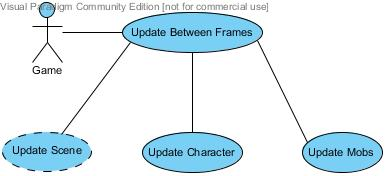
\includegraphics[width=140mm]{UML_Diagram/Use_Case/Game_Process.jpg}
					\caption{Update process between frames}
					\end{figure}
					
					\begin{figure}[H]
					\centering
					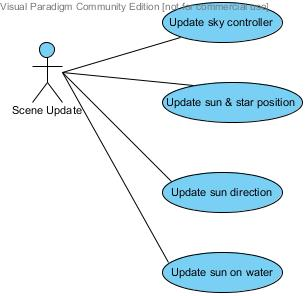
\includegraphics[width=140mm, height=100mm]{UML_Diagram/Use_Case/Update_Scene.jpg}
					\caption{Update of scene elements}
					\end{figure}
					
					\begin{figure}[H]
					\centering
					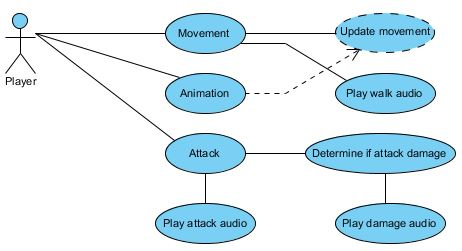
\includegraphics[width=140mm]{UML_Diagram/Use_Case/Player_Actions.jpg}
					\caption{Actions available to player}
					\end{figure}
					
					\begin{figure}[H]
					\centering
					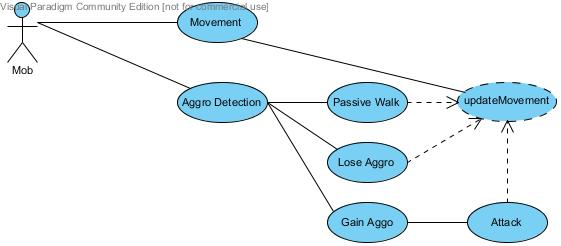
\includegraphics[width=140mm]{UML_Diagram/Use_Case/Mob_Actions.jpg}
					\caption{Actions available to mobs}
					\end{figure}
					
				\vspace{0.2in}
				\subsubsection*{User-interface Diagrams:}
				\addcontentsline{toc}{subsubsection}{User-interface Diagrams}
				\vspace{0.2in}
				
					\begin{figure}[H]
					\centering
					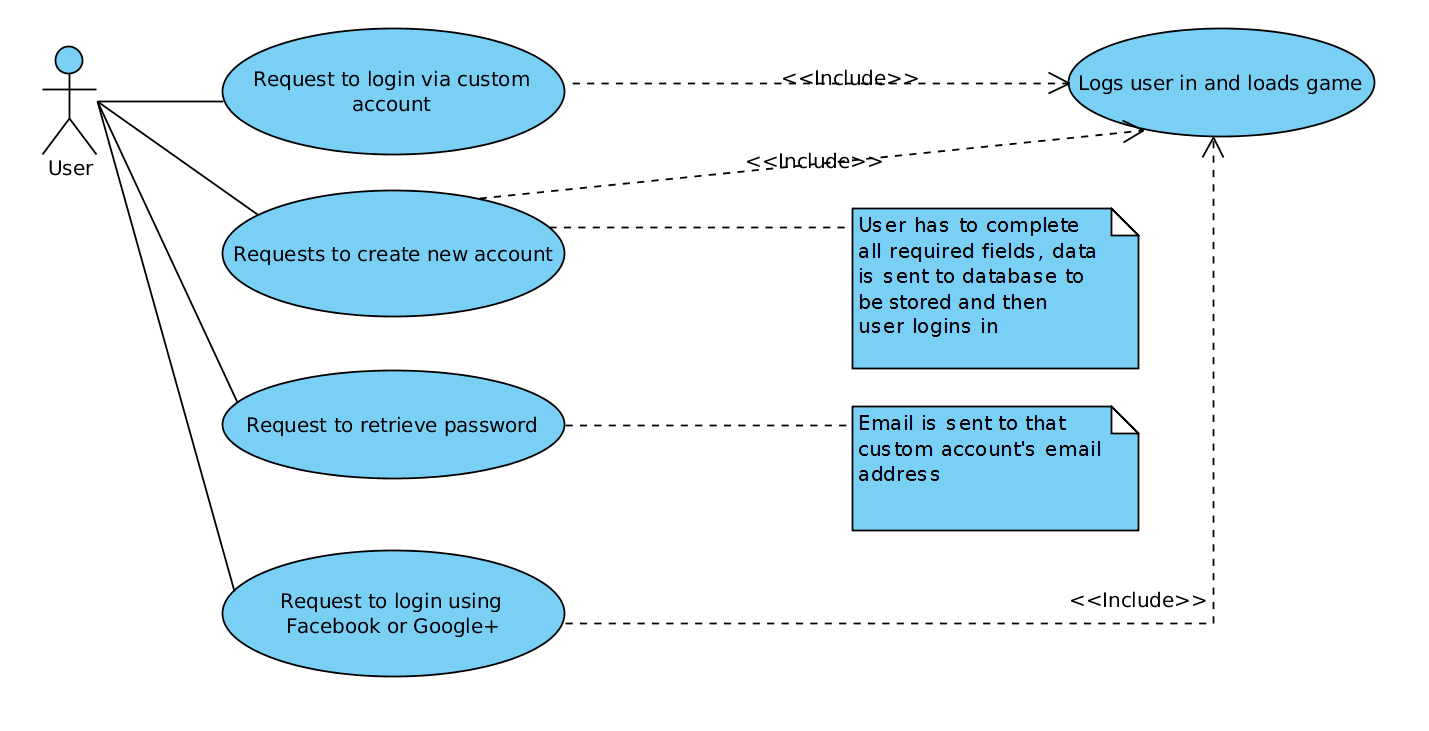
\includegraphics[width=140mm]{UML_Diagram/Use_Case/User_Login.jpg}
					\caption{User Login Screen}
					\end{figure}
				
					\begin{figure}[H]
					\centering
					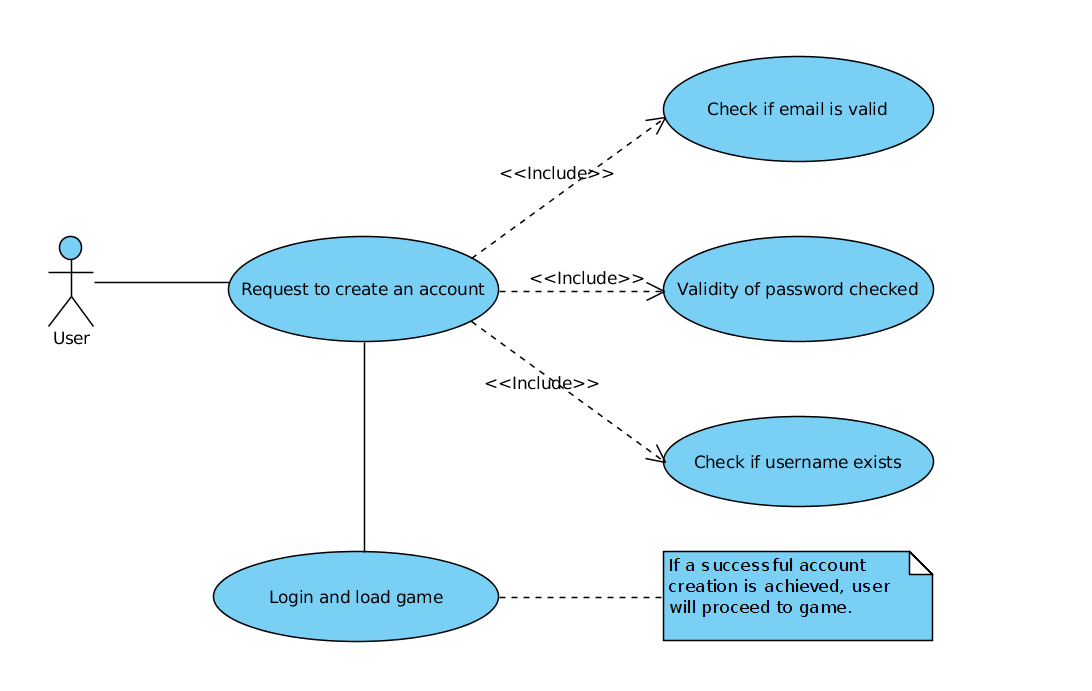
\includegraphics[width=140mm]{UML_Diagram/Use_Case/CreatAccount_UseCase.jpg}
					\caption{Create New Account Screen}
					\end{figure}
				
					\begin{figure}[H]
					\centering
					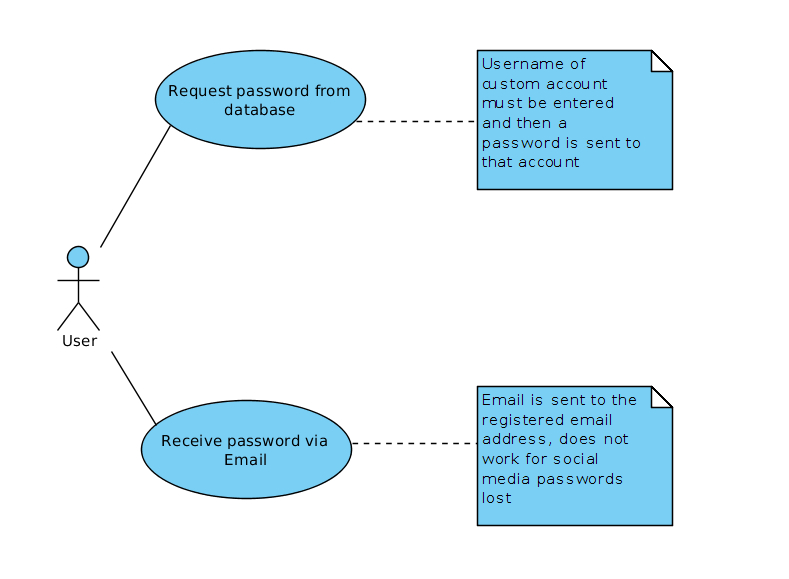
\includegraphics[width=140mm]{UML_Diagram/Use_Case/RetrievePassword_UseCase.jpg}
					\caption{Retrieve Password Screen}
					\end{figure}
				
					\begin{figure}[H]
					\centering
					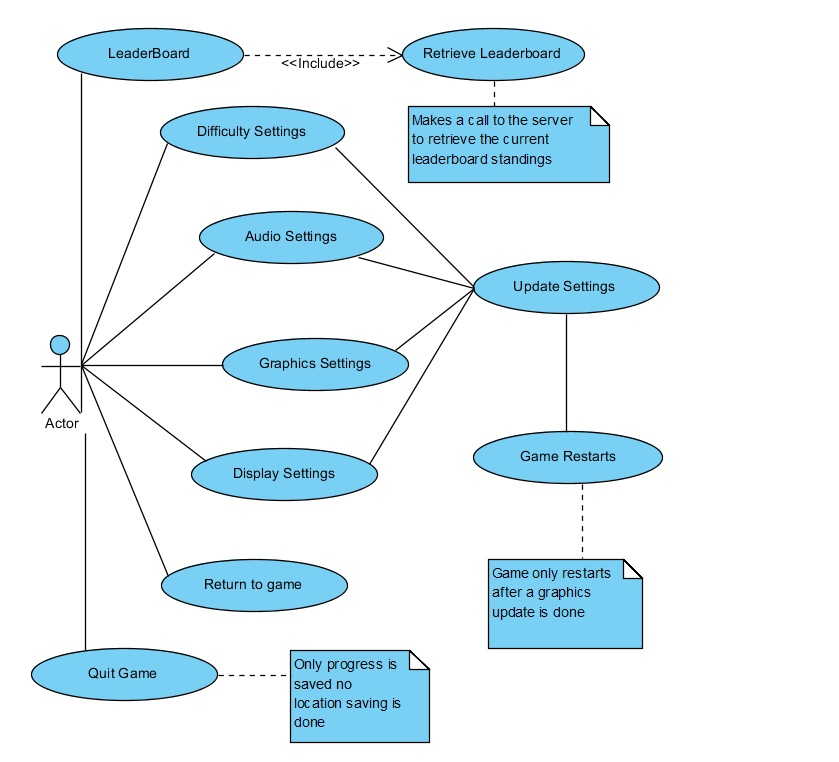
\includegraphics[width=140mm]{UML_Diagram/Use_Case/OptionsScreen_UseCase.jpg}
					\caption{Options Screen}
					\end{figure}
				
				\begin{figure}[H]
					\centering
					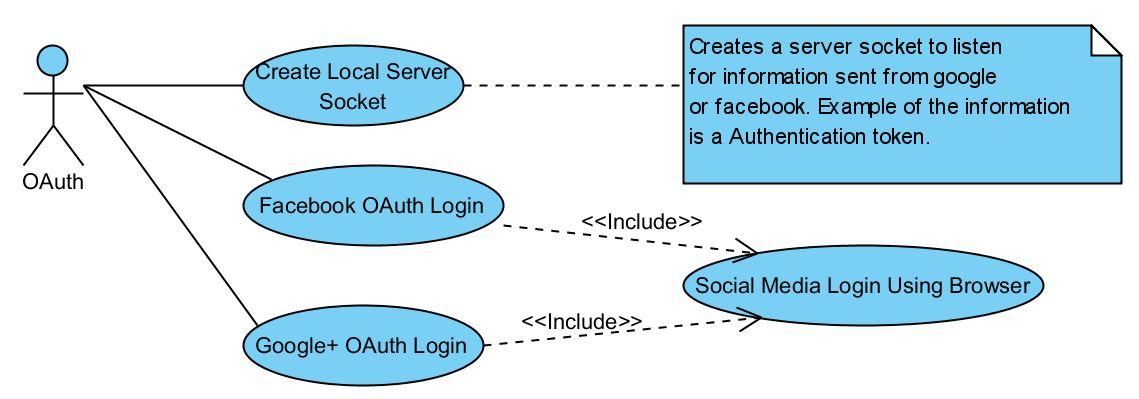
\includegraphics[width=140mm]{UML_Diagram/Use_Case/OAuth.jpg}
					\caption{Login using social media(OAuth)}
					\end{figure}
				
				\vspace{0.2in}
				\subsubsection*{Server Diagrams:}
				\addcontentsline{toc}{subsubsection}{Server Diagrams}
				\vspace{0.2in}
				
					\begin{figure}[H]
					\centering
					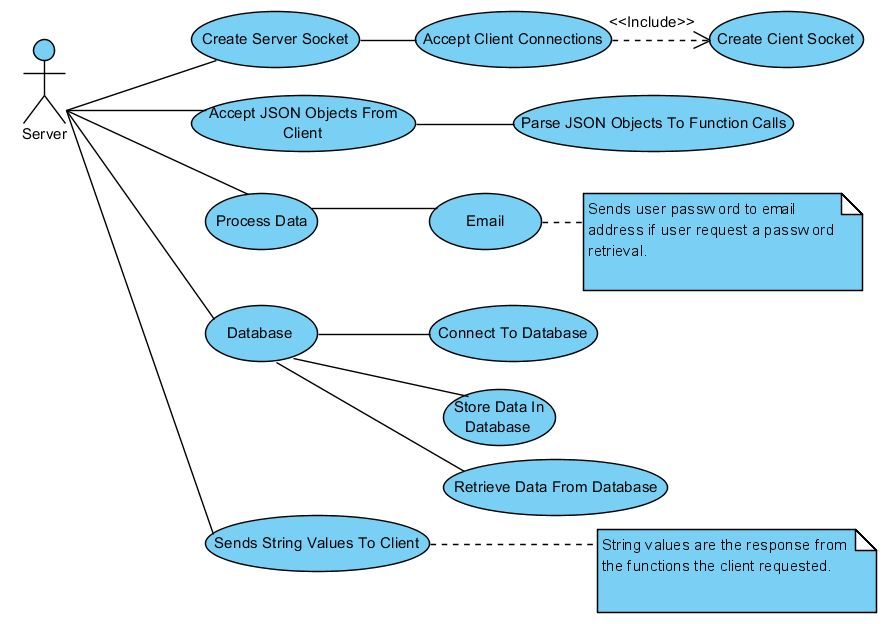
\includegraphics[width=140mm]{UML_Diagram/Use_Case/Server.jpg}
					\caption{Server Functionality}
					\end{figure}
					
					\begin{figure}[H]
					\centering
					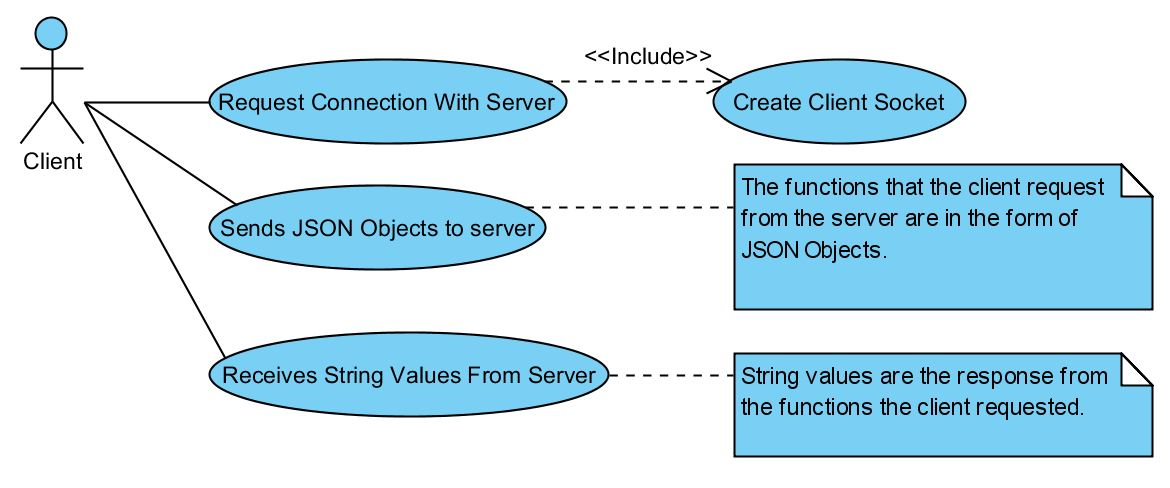
\includegraphics[width=140mm]{UML_Diagram/Use_Case/Client.jpg}
					\caption{User Interaction With Server}
					\end{figure}
				
			\vspace{0.2in}
			\subsection*{Use Case prioritization:}
			\addcontentsline{toc}{subsection}{Use Case prioritization / services contracts}
			\vspace{0.1in}
					
				\subsubsection*{Critical:}
				\addcontentsline{toc}{subsubsection}{Critical}
				\vspace{0.1in}
					
					\begin{itemize}
						\item Update process between frames.
						\item Update of scene elements.
						\item Server Functionality.
						\item User Interaction With Server.
						\item Login using custom login.
						\item Create a new custom account.	
						\item Leaderboard of best all players and scores.					
					\end{itemize}	
					
				\vspace{0.2in}
				\subsubsection*{Important:}
				\addcontentsline{toc}{subsubsection}{Important}
				\vspace{0.2in}
				
					\begin{itemize}
						\item Actions available to player.
						\item Actions available to mobs.
						\item Login using social media(OAuth).
						\item Retrieval of password.
						\item Can change the graphical settings of the game.
						\item Can change audio settings.
						\item Have password encryption through the entire game.
					\end{itemize}
				
				\vspace{0.2in}
				\subsubsection*{Nice-To-Have:}
				\addcontentsline{toc}{subsubsection}{Nice-To-Have}
				\vspace{0.2in}
					\begin{itemize}
						\item Update the grpahics while game running.
						\item Change of difficulty settings.
						\item Modibility of the game from external sources.
						\item Addition of more maps.
						\item Multiple types of zombies.
						\item Audit and error log.
					\end{itemize}
					
			\vspace{0.2in}
			\subsection*{Use Case services contracts:}
			\addcontentsline{toc}{subsection}{Use Case prioritization / services contracts}
			\vspace{0.1in}
				
				\subsubsection*{Game Diagrams:}
				\addcontentsline{toc}{subsubsection}{Game Diagrams}
				\vspace{0.1in}
					
					\hspace{5mm}Update process between frames
					\begin{itemize}
						\item Pre-Conditions: \\
							Game is still running within the main game loop. \\
							Update time is provided from game engine defining the uptime of game. \\
							Player character is not null and initialized to be update. \\
							Mob characters is not null and initialized to be update.
						\item Post-Conditions: \\
							Game scene has updated as defined in update scene elements. \\
							Character action updated as defined in actions of player. \\
							Mobs actions updated as defined in actions of mob.
						\item Request and Results Data Structures \\
							
					\end{itemize}
					
					\vspace{0.1in}
					Actions available to player
					\begin{itemize}
						\item Pre-Condition: \\
							Character handler is not null and initialized. \\
							Character repositioning direction available from the directional keys pressed. \\
							Player animations channel is retrieved from model and can be updated. \\
							Player attack registered for process.
						\item Post-Condition: \\
							Character position has been updated according to direction of movement and movement speed. \\
							Player animation has been set successfully to animations channel with define loop state and play speed. \\
							Player attack action has occurred and processed between player and attacked mob.
						\item Request and Results Data Structures \\
							
					\end{itemize}
					
					\vspace{0.1in}
					Actions available to mobs
					\begin{itemize}
						\item Pre-Condition: \\
							Character handler is not null and initialized. \\
							Character repositioning direction is given from players position. \\
							Mob aggro detection is not null and attach to physics space. \\
							Mob aggro obtained flagged. \\
							Mob aggro loss flagged. \\
							Mob animation channel is retrieved from model and can be updated. \\
							Mob attack registered for process.
						\item Post-Condition: \\
							Character position updated to the direction of player and a distance of the movement speed. \\
							Mob aggro process and state updated for motion and animation loop. \\
							Mob animation has been set successfully to animations channel with define loop state and play speed. \\
							Mob attack action has occurred and processed between mob and player.
						\item Request and Results Data Structures \\
						
					\end{itemize}
					
					\vspace{0.1in}
					Update of scene elements
					\begin{itemize}
						\item Pre-Condition: \\
							Sky control not null and initialized. \\
							Update value provided from game engine of frame time.
						\item Post-Condition: \\
							Sun \& Stars updated by sky control. \\
							Sun direction updated retrieved from sky control and assigned to the light. \\
							Sun on the water updated from the new set light direction. \\
							Time of day updated through sky control.
						\item Request and Results Data Structures \\
						
					\end{itemize}
					
				\vspace{0.2in}
				\subsubsection*{User-interface Diagrams:}
				\addcontentsline{toc}{subsubsection}{User-interface Diagrams}
				\vspace{0.2in}
				
				\vspace{0.1in}
					\hspace{5mm}Creating a custom account
					\begin{itemize}
						\item Pre-Condition: \\
							Client connection to server must be created. \\
							User must not have an existing account registered to the email address he wants to use. \\
							 The username must not be taken by any other player. \\
						\item Post-Condition: \\				
							User must be logged into the game. \\
							User's details must be stored to the database. \\
							User's username and score must be displayed on the leaderboard. 
						\item Request and Results Data Structures \\
						
					\end{itemize}
					
				\vspace{0.1in}Login using a custom account
					\begin{itemize}
						\item Pre-Condition: \\
							Client connection to server must be created. \\				
							User must have a registered custom account. \\
						\item Post-Condition: \\
							User must be logged in and game must be running. \\
							Username must be displayed on the leaderboard. \\			
						\item Request and Results Data Structures \\
						
					\end{itemize}

				\vspace{0.1in}Retrieval of custom account password
					\begin{itemize}
						\item Pre-Condition: \\
							Client connection to server must be created. \\
							User must have a registerd username and email linked to their custom account. \\ 
						\item Post-Condition: \\
							Email is sent to registered email address. \\
							User is taken back to the login screen. \\
						\item Request and Results Data Structures \\
						
					\end{itemize}
									
				\vspace{0.1in}Leaderboard updates
					\begin{itemize}
						\item Pre-Condition: \\
							User must be logged in. \\ 
							User must kill a zombie. \\
						\item Post-Condition: \\
							Score updated on leaderboard screen. \\						
						\item Request and Results Data Structures \\
						
					\end{itemize}					
														
				\vspace{0.1in}Loading Screen
					\begin{itemize}
						\item Pre-Condition: \\
							User must have a successful login. \\
						\item Post-Condition: \\
						 	Game is loaded and user can play. \\
						\item Request and Results Data Structures \\
						
					\end{itemize}	
								
				\vspace{0.1in}Options Menu
					\begin{itemize}
						\item Pre-Condition: \\
							User must be logged into the game. \\
							User must hit the escape key. \\
						\item Post-Condition: \\
							Options menu screen must appear. \\
							Mouse must be visible. \\
							Selections must be selectable. \\
						\item Request and Results Data Structures \\
						
					\end{itemize}	
									
				\vspace{0.1in}Graphics Settings tab
					\begin{itemize}
						\item Pre-Condition: \\
							Options Menu must be open. \\
							Graphics settings must be selected. \\
						\item Post-Condition: \\
							Graphics settings are displayed. \\
							Previous choices must be already ticked. \\
						\item Request and Results Data Structures \\
						
					\end{itemize}
									
				\vspace{0.1in}Display Settings tab
					\begin{itemize}
						\item Pre-Condition: \\
							Options Menu must be open. \\
							Display settings must be selected. \\
						\item Post-Condition: \\
							Display settings are displayed. \\
						\item Request and Results Data Structures \\
						
					\end{itemize}
									
				\vspace{0.1in}Audio Settings tab
					\begin{itemize}
						\item Pre-Condition: \\
							Options Menu must be open. \\
							Audio settings must be selected. \\
						\item Post-Condition: \\
							Audio settings are displayed. \\
							Previous volumes must be loaded. \\
						\item Request and Results Data Structures \\
						
					\end{itemize}
									
				\vspace{0.1in}Leaderboard tab
					\begin{itemize}
						\item Pre-Condition: \\
							Options Menu must be open. \\
							Leaderboard must be selected. \\
						\item Post-Condition: \\
							Leaderboard is displayed. \\
						\item Request and Results Data Structures \\
						
					\end{itemize}									
									
				\vspace{0.1in}Quiting the game
					\begin{itemize}
						\item Pre-Condition: \\
							User must be in the options menu or login screen. \\
							User must select quit game. \\ 
						\item Post-Condition: \\
							Game must close and user returned to previous position on desktop. \\
						\item Request and Results Data Structures \\
						
					\end{itemize}
														
				
				\vspace{0.1in}Login using social media(OAuth)
					\begin{itemize}
						\item Pre-Condition: \\
							User must have a google or facebook account. \\
							User must login with his facebook or google profile. \\
							User must grant permission for the game to access social information.
						\item Post-Condition: \\
							User must be logged in the game. \\
							Server must have an access token of the social media used to log in.			
						\item Request and Results Data Structures \\
						
					\end{itemize}
				
				\newpage
				\subsubsection*{Server Diagrams:}
				\addcontentsline{toc}{subsubsection}{Server Diagrams}
				
				\vspace{0.1in}
					\hspace{5mm}Server Functionality
					\begin{itemize}
						\item Pre-Condition: \\
							Server socket needs to be created. \\
							Connection from server to database needs to be established. \\
							Server needs to listen for incoming connection.
						\item Post-Condition: \\
							Server needs to accept all incoming connection from the game. \\
							Server must handle all functions requested from user(game).\\
							Server needs to store and retrieve data from the database.			
						\item Request and Results Data Structures \\
							All function request from the user(game) are JSON strings. 
						
					\end{itemize}
					
					\vspace{0.1in}
					User Interaction With Server
					\begin{itemize}
						\item Pre-Condition: \\
							Client socket needs to be created. \\
							Client socket must connect with server. \\
							Client needs to send data to the server. 
						\item Post-Condition: \\
							Client must be connected to server. \\
							Client needs to receive data from server.			
						\item Request and Results Data Structures \\
							All data sent and received between server and client are JSON strings.						
					\end{itemize}
					
			\vspace{0.2in}
			\subsection*{Process specifications:}
			\addcontentsline{toc}{subsection}{Process specifications}
			\vspace{0.1in}
			
				\subsubsection*{Game Diagrams:}
				\addcontentsline{toc}{subsubsection}{Game Diagrams}
				\vspace{0.1in}
					
					\begin{figure}[H]
					\centering
					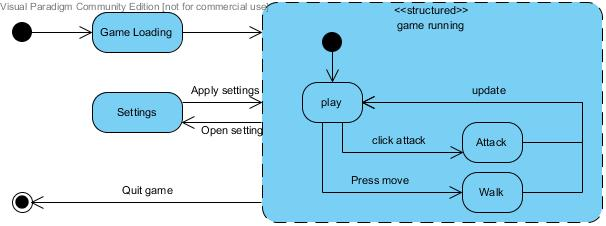
\includegraphics[width=180mm, height=50mm]{UML_Diagram/Activity/GameUpdate_Activity.jpg}
					\caption{Main game activity}
					\label{overflow}
					\end{figure}
					
					\begin{figure}[H]
					\centering
					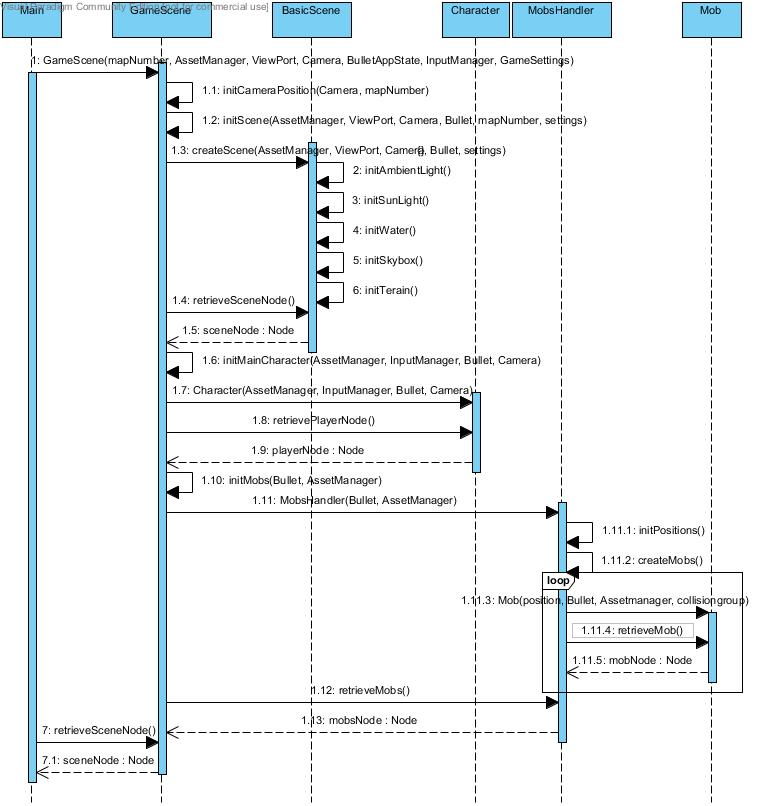
\includegraphics[width=180mm, height=150mm]{UML_Diagram/Sequence/Game_Creation.jpg}
					\caption{Game Creation}
					\label{overflow}
					\end{figure}
					
					The entire process to create all the game aspects after a successful login:
					\begin{itemize}
						\item 1.1 Takes the game camera and positions it accordingly to which map is used.
						\item 1.2 Creates basic scene with the required map, calls 1.3 and 1.4.
						\item 2 Creates the scene ambient light with the required colour and intensity.
						\item 3 Creates the sun light with colour and intensity, which will be bound to SkyControl is in use.
						\item 4 Will determine if basic water or post processing water is in use. Basic water is a plane with scene reflection and simple motion. Post processed water has higher transparency, smoother motion and foam at the sea shore.
						\item 5 Will determine if basic skybox or SkyControl should be used. Basic skybox is a box with textures placed on. SkyControl create 2 spheres, 1 with the star system and the other the sky colour and moon/sun. It controls the motion of the sun, moon, stars and the second sphere turns transparent at day night changes.
						\item 6 Load the required scene which contains the terrain and trees. It adds a rigigbody controller to the terrain for collision control and creates a cubic collision box for each individual tree.
						\item 1.7 Detailed in a later diagram.
						\item 1.11.1 Initializes all the positions where mobs will be placed through out the scene.
						\item 1.11.3 Details in a later diagram.
					\end{itemize}
					
					\begin{figure}[H]
					\centering
					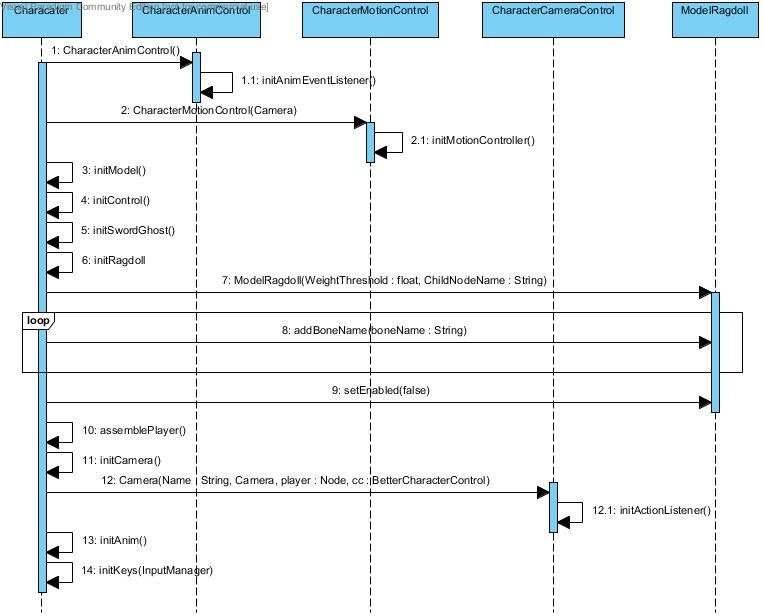
\includegraphics[width=160mm, height=90mm]{UML_Diagram/Sequence/Player_Creation.jpg}
					\caption{Creation of player model}
					\label{overflow}
					\end{figure}
					
					The process of creating the model that the user will be controlling:
					\begin{itemize}
						\item 1.1 Creates the AnimEventListener that is called at the end of an animation cycle and when the animation is changed.
						\item 2.1 Creates the ActionListener that is called on key presses and mouse clicks which send the corresponding action name through required to determine in which direction the player is moving or if he is attacking.
						\item 3 Loads the model through the asset manager, sets the node name, set its starting position and in with direction is it looking in regards to the camera.
						\item 4 Creates the BetterCharacterControl which is bound to the player, this controller has a size defined collision box around the player, controls all the affected forces on the player and moves the model to where it is repositioned on movement.
						\item 5 Creates a Ghost collision box around the sword which will trigger a collision event when it passes through another collision box. The collision group it is bound to is set as well as with which groups this box can collide with.
						\item 7 Creates the Ragdoll controller that will be triggered on player death.
						\item 10 Adds all the created controllers to the player node and to the physics controller.
						\item 12 Creates a camera node what will create the pivot required for mouse movement.
						\item 12.1 Initializes the AnalogListener that will trigger on mouse movement and route the camera around the required axis with a defined speed.
						\item 13 Retrieves the animation controller for the model containing the created animation, attaches the animation listener to the controller, creates a channel to play animations and sets the animation to the default standing animation.
						\item 14 Sets up all the keys and mouse movement triggers with their corresponding listeners and action names.
					\end{itemize}
					
					\begin{figure}[H]
					\centering
					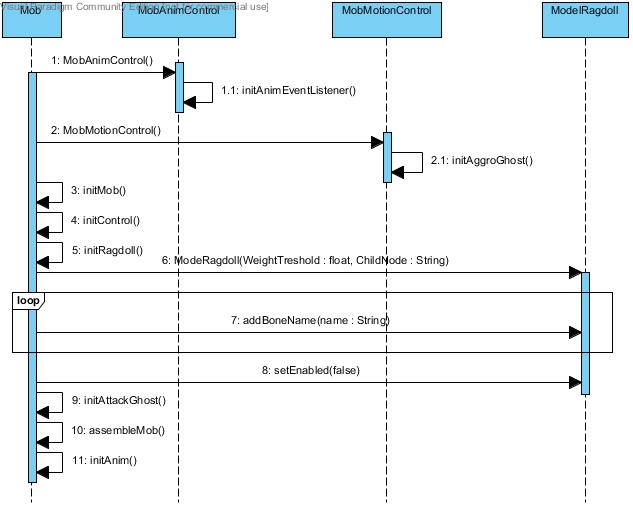
\includegraphics[width=160mm, height=90mm]{UML_Diagram/Sequence/Mob_Creation.jpg}
					\caption{Mob creation}
					\label{overflow}
					\end{figure}
					
					The process of creating the model that will be used for all enemies:
					\begin{itemize}
						\item 1.1 Creates the AnimEventListener that is called at the end of an animation cycle and when the animation is changed.
						\item 2.1 Creates the ghost controller that will be used to determine is a player has entered that detection range of a mob where aggro is obtained. When aggro is lost it will determined if it is regain able while moving toward its passive position.
						\item 3 Loads the model through the asset manager, sets the node name and set its passive position.
						\item 4 Creates the BetterCharacterControl which is bound to the player, this controller has a size defined collision box around the player, controls all the affected forces on the player and moves the model to where it is repositioned on movement.
						\item 6 Creates the Ragdoll controller that will be triggered on player death.
						\item 9 Creates a Ghost collision box around the mobs hand which will trigger a collision event when it passes through another collision box. The collision group it is bound to is set as well as with which groups this box can collide with.
						\item 10 Adds all the created controllers to the mob node and to the physics controller.
						\item 11 Retrieves the animation controller for the model containing the created animation, attaches the animation listener to the controller, creates a channel to play animations and sets the animation to the default standing animation.
					\end{itemize}
					
					\begin{figure}[H]
					\centering
					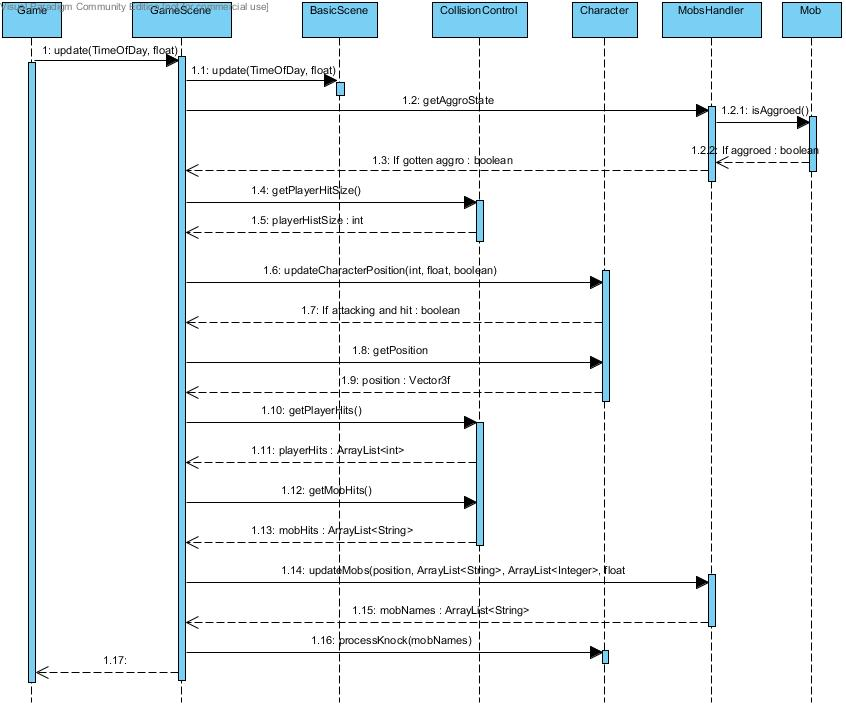
\includegraphics[width=180mm, height=105mm]{UML_Diagram/Sequence/Update_Sequence.jpg}
					\caption{Update process between frames}
					\label{overflow}
					\end{figure}
					
					These is a detailed process depiction of game updates that happens between each frame. Detail diagrams for player and mob updates follow as state diagrams.
					
					\begin{figure}[H]
					\centering
					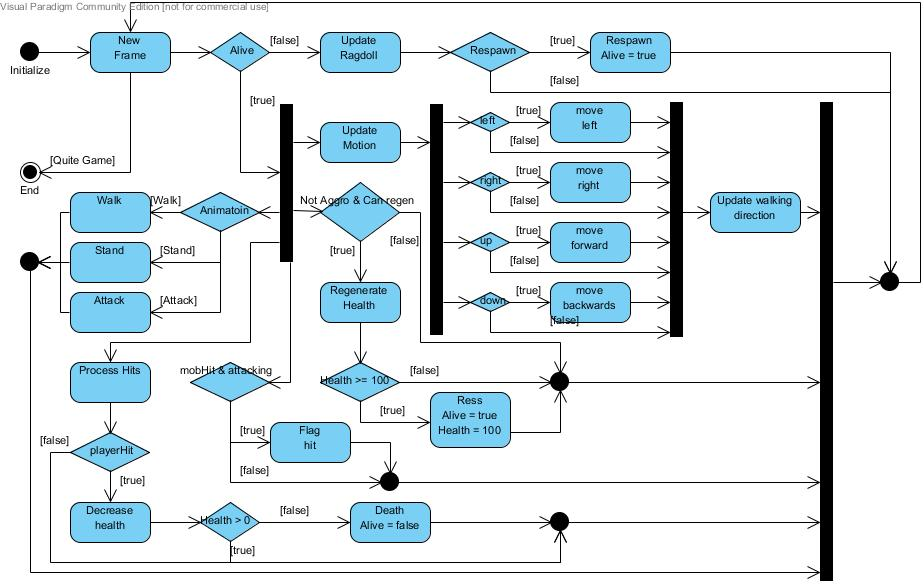
\includegraphics[width=180mm, height=80mm]{UML_Diagram/State/Player_State.jpg}
					\caption{Player update state cycle}
					\label{overflow}
					\end{figure}
					
					This diagram depicts all the active states and decisions the player goes through on frame draw. From motion and animation updates, to health loss and regeneration and attacks.
					
					\begin{figure}[H]
					\centering
					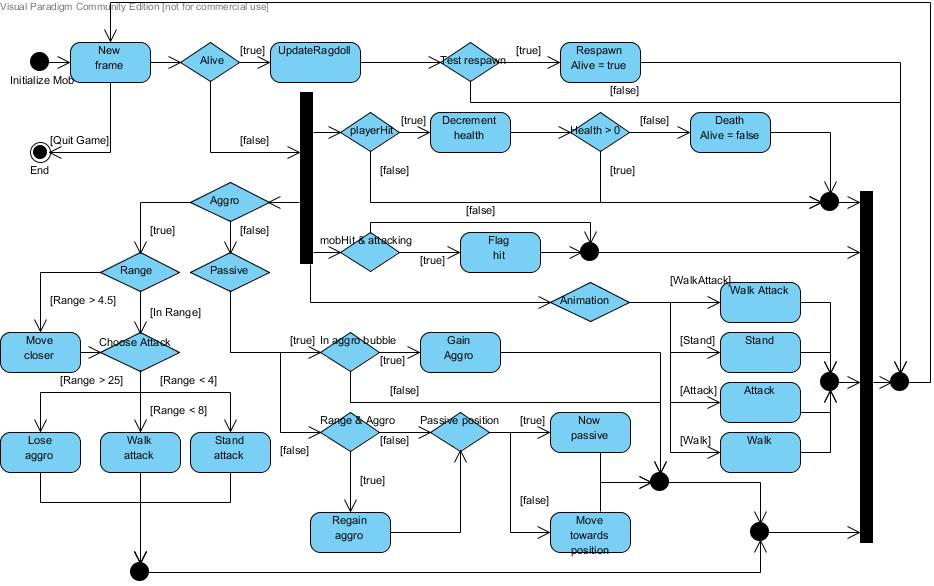
\includegraphics[width=180mm, height=80mm]{UML_Diagram/State/Mob_State.jpg}
					\caption{Enemy update state cycle}
					\label{overflow}
					\end{figure}
					
					This diagram depicts all the active states and decisions a single mob as to go through at each new frame draw. From death and animation updates, aggression detections, motion and attack decisions.
			
				\subsubsection*{User-Interface Diagrams:}
				\addcontentsline{toc}{subsubsection}{UI Diagrams}
				\vspace{0.1in}
				
					\begin{figure}[H]
					\centering
					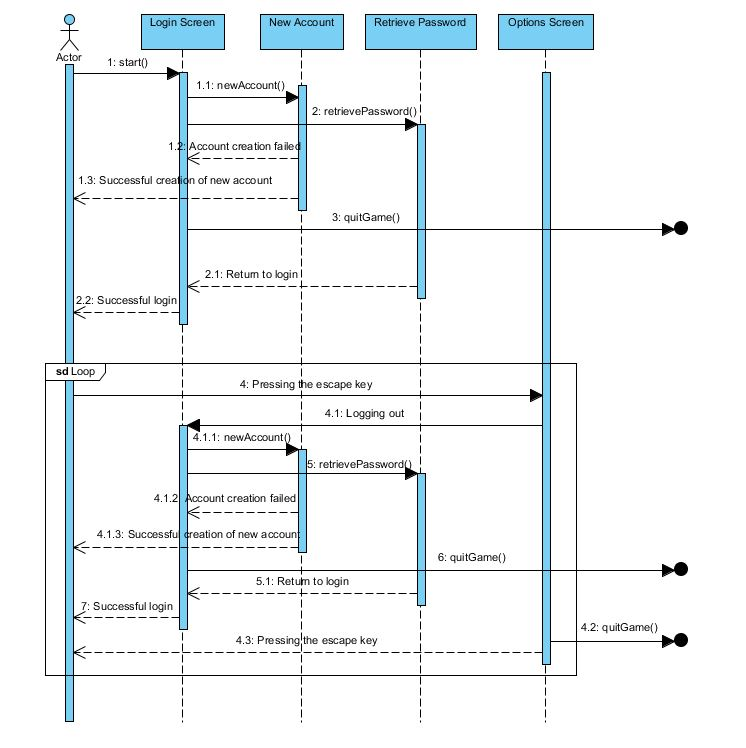
\includegraphics[width=180mm]{UML_Diagram/Sequence/GUI_Screens.jpg}
					\caption{User-Interface cycle}
					\label{overflow}
					\end{figure}
					
					\begin{figure}[H]
					\centering
					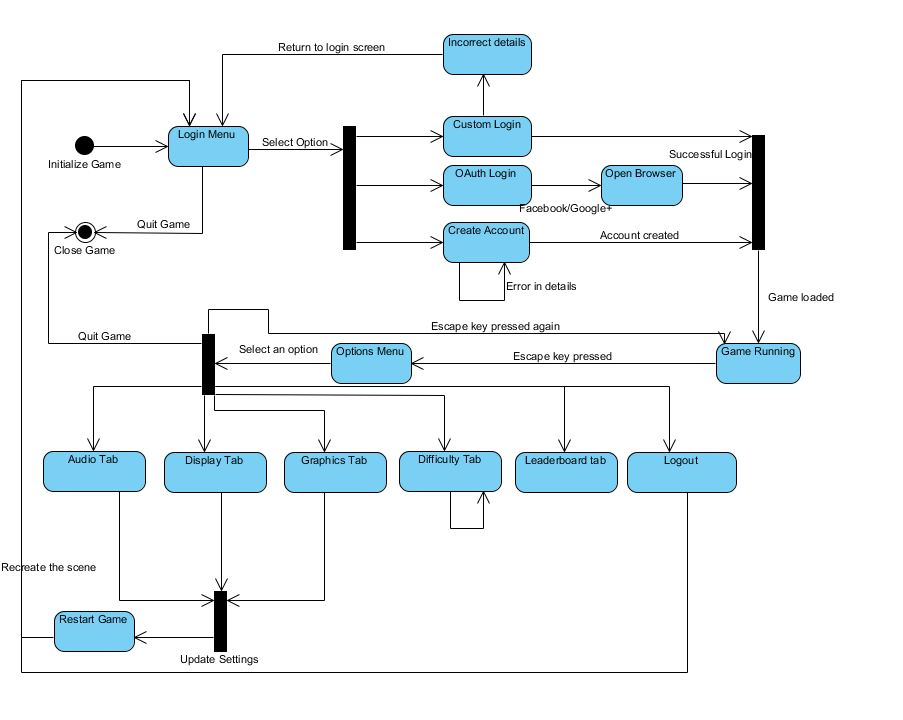
\includegraphics[width=180mm]{UML_Diagram/State/GUI_State.jpg}
					\caption{User-Interface cycle}
					\label{overflow}
					\end{figure}
					
					\begin{figure}[H]
					\centering
					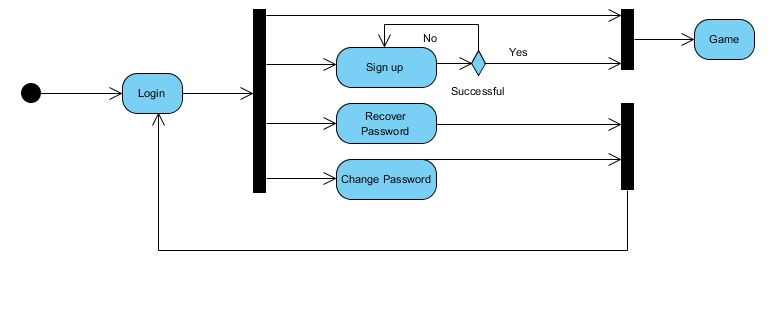
\includegraphics[width=180mm]{UML_Diagram/Activity/login.jpg}
					\caption{User-Interface login screen}
					\label{overflow}
					\end{figure}
					
					\begin{figure}[H]
					\centering
					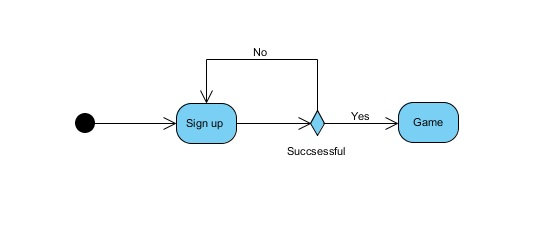
\includegraphics[width=180mm]{UML_Diagram/Activity/signup.jpg}
					\caption{User-Interface sign up screen}
					\label{overflow}
					\end{figure}
					
					\begin{figure}[H]
					\centering
					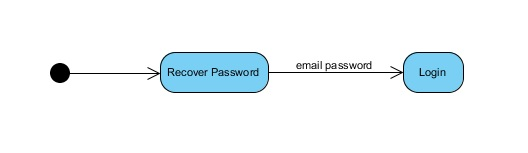
\includegraphics[width=180mm]{UML_Diagram/Activity/recoverpassword.jpg}
					\caption{User-Interface recover password screen}
					\label{overflow}
					\end{figure}
					
					\begin{figure}[H]
					\centering
					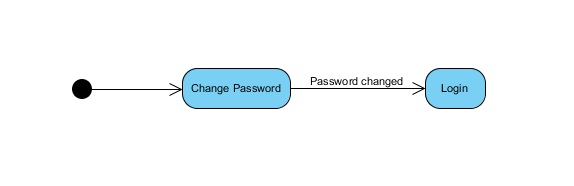
\includegraphics[width=180mm]{UML_Diagram/Activity/changepassword.jpg}
					\caption{User-Interface change password screen}
					\label{overflow}
					\end{figure}
					
					\begin{figure}[H]
					\centering
					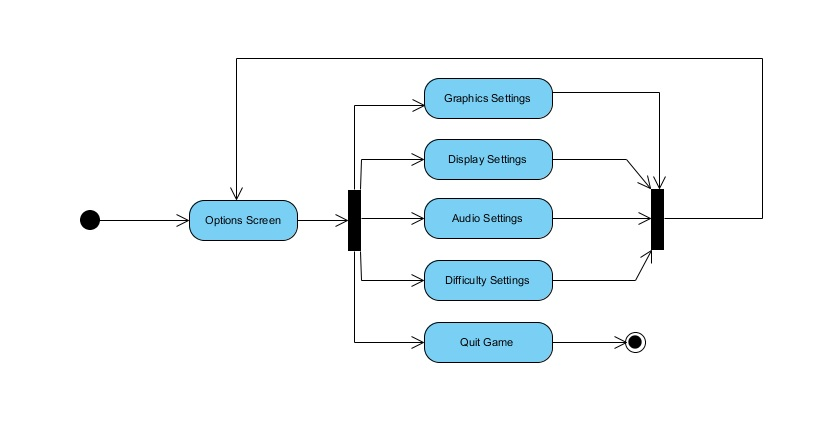
\includegraphics[width=180mm]{UML_Diagram/Activity/optionsscreen.jpg}
					\caption{User-Interface options menu screen}
					\label{overflow}
					\end{figure}
				
				\subsubsection*{Server Diagrams:}
				\addcontentsline{toc}{subsubsection}{Server Diagrams}
				\vspace{0.1in}
				
					\begin{figure}[H]
					\centering
					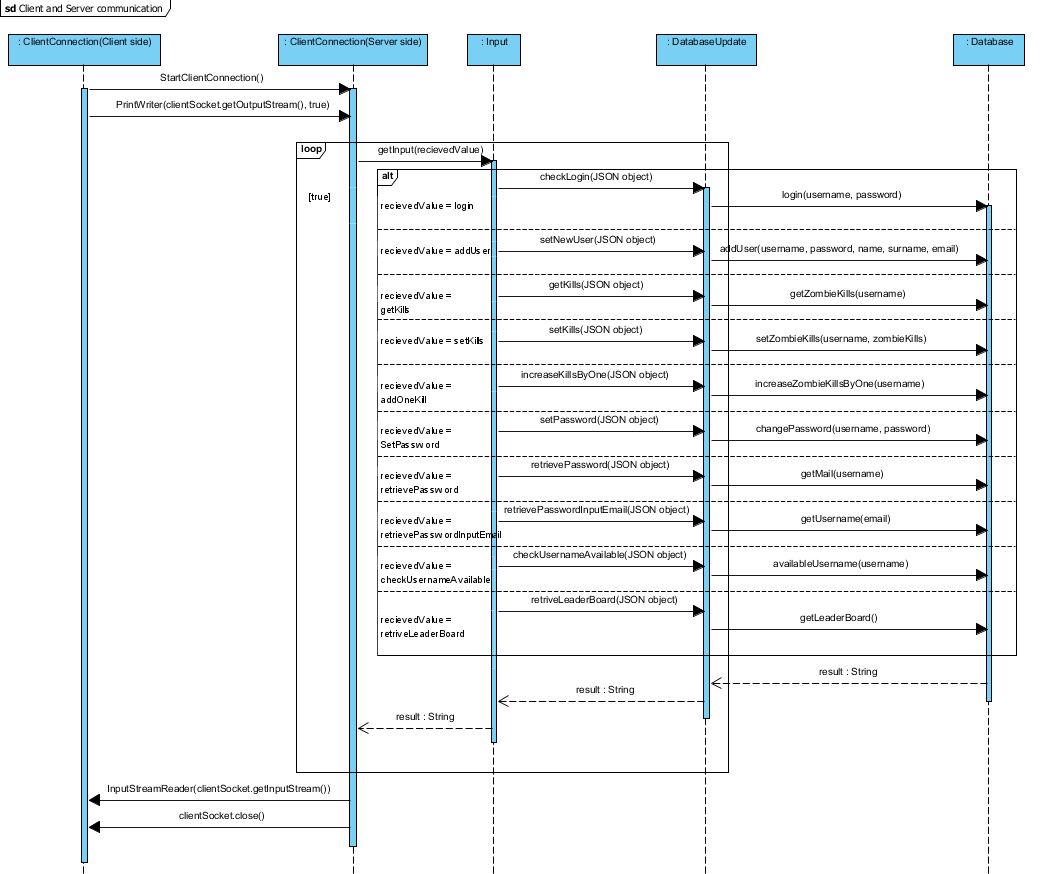
\includegraphics[width=180mm]{UML_Diagram/Sequence/Client_Server_Sequence_Diagram.jpg}
					\caption{Client and Server communication sequence diagram}
					\label{overflow}
					\end{figure}
			
					\begin{figure}[H]
					\centering
					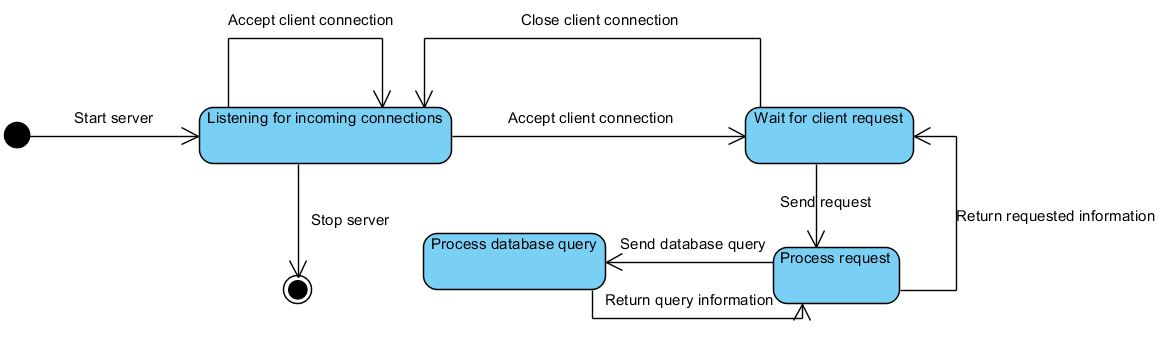
\includegraphics[width=180mm]{UML_Diagram/State/Server_State_Diagram.jpg}
					\caption{Server cycle}
					\label{overflow}
					\end{figure}
			
			\vspace{0.2in}
			\subsection*{Domain Objects:}
			\addcontentsline{toc}{subsection}{Domain Objects}
			\vspace{0.1in}
			
				\vspace{0.2in}
				\subsubsection*{Class Diagrams:}
				\addcontentsline{toc}{subsubsection}{Class Diagrams}
				\vspace{0.1in}
				
					\begin{figure}[H]
					\centering
					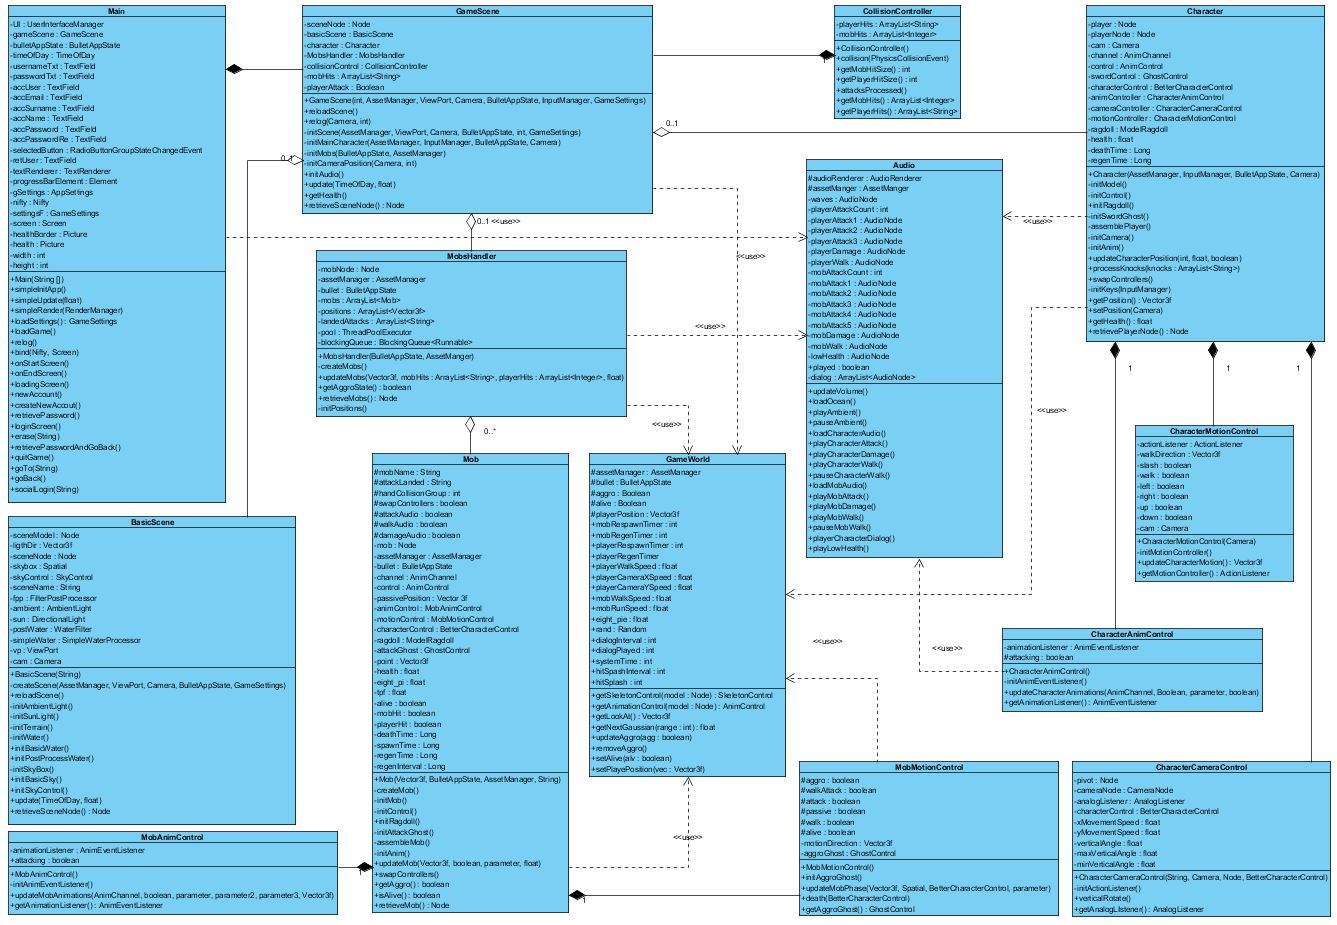
\includegraphics[width=180mm]{UML_Diagram/Class/Game_Classes.jpg}
					\caption{Game level class diagram}
					\label{overflow}
					\end{figure}
					
					\begin{figure}[H]
					\centering
					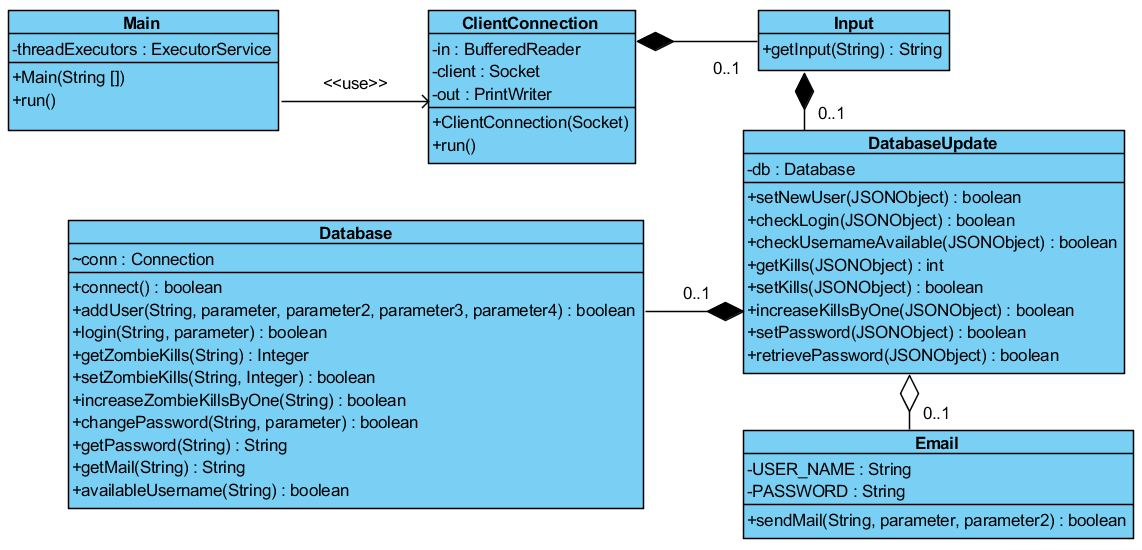
\includegraphics[width=180mm]{UML_Diagram/Class/Server_Classes.jpg}
					\caption{Server level class diagram}
					\label{overflow}
					\end{figure}
					
					\begin{figure}[H]
					\centering
					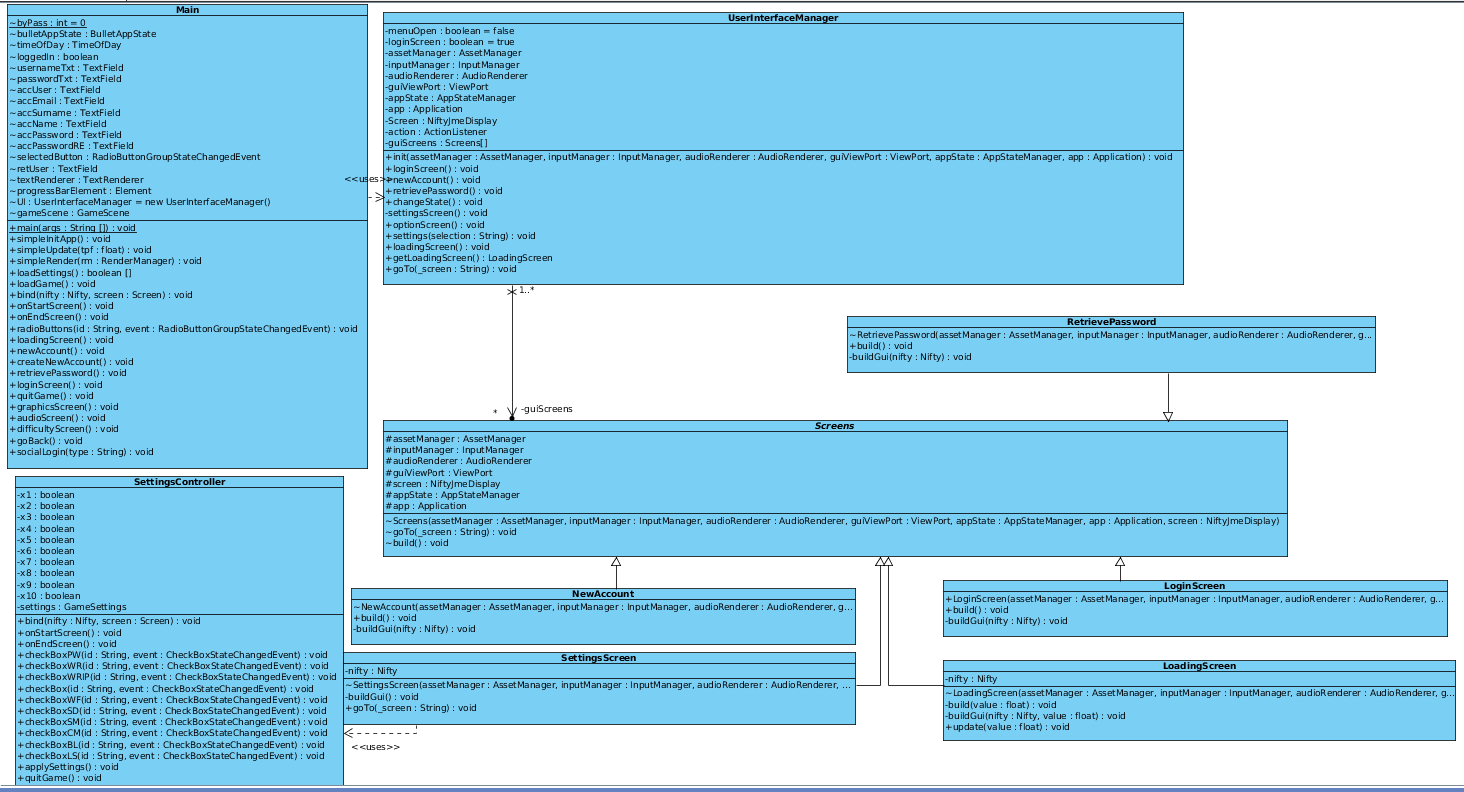
\includegraphics[width=180mm]{UML_Diagram/Class/GUI_Classes.jpg}
					\caption{User-Interface class diagram}
					\label{overflow}
					\end{figure}
					
				\vspace{0.2in}	
				\subsubsection*{ERD Diagrams:}
				\addcontentsline{toc}{subsubsection}{ERD Diagrams}
				\vspace{0.1in}
				
					\begin{figure}[H]
					\centering
					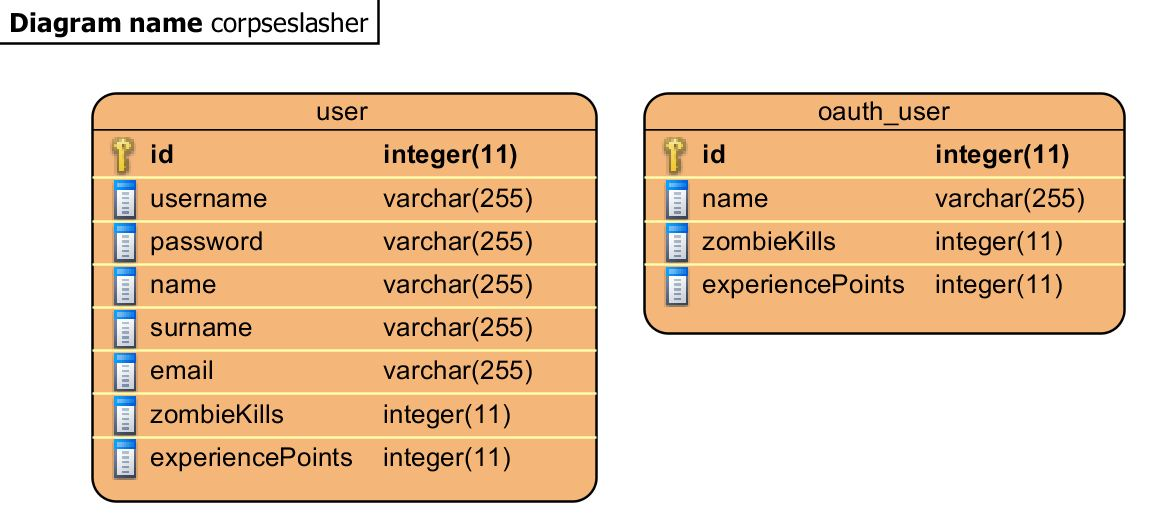
\includegraphics[width=180mm]{UML_Diagram/ERD/Database.jpg}
					\caption{Database ERD diagram}
					\label{overflow}
					\end{figure}
					
					
		\vspace{0.2in}
		
		\section*{\colorbox{blue}{\makebox[\textwidth-2\fboxsep][l]{\bfseries\color{white} Application Design }}} \addcontentsline{toc}{section}{Application Design}
		\vspace{0.1in}
		
		\begin{figure}[H]
		\centering
		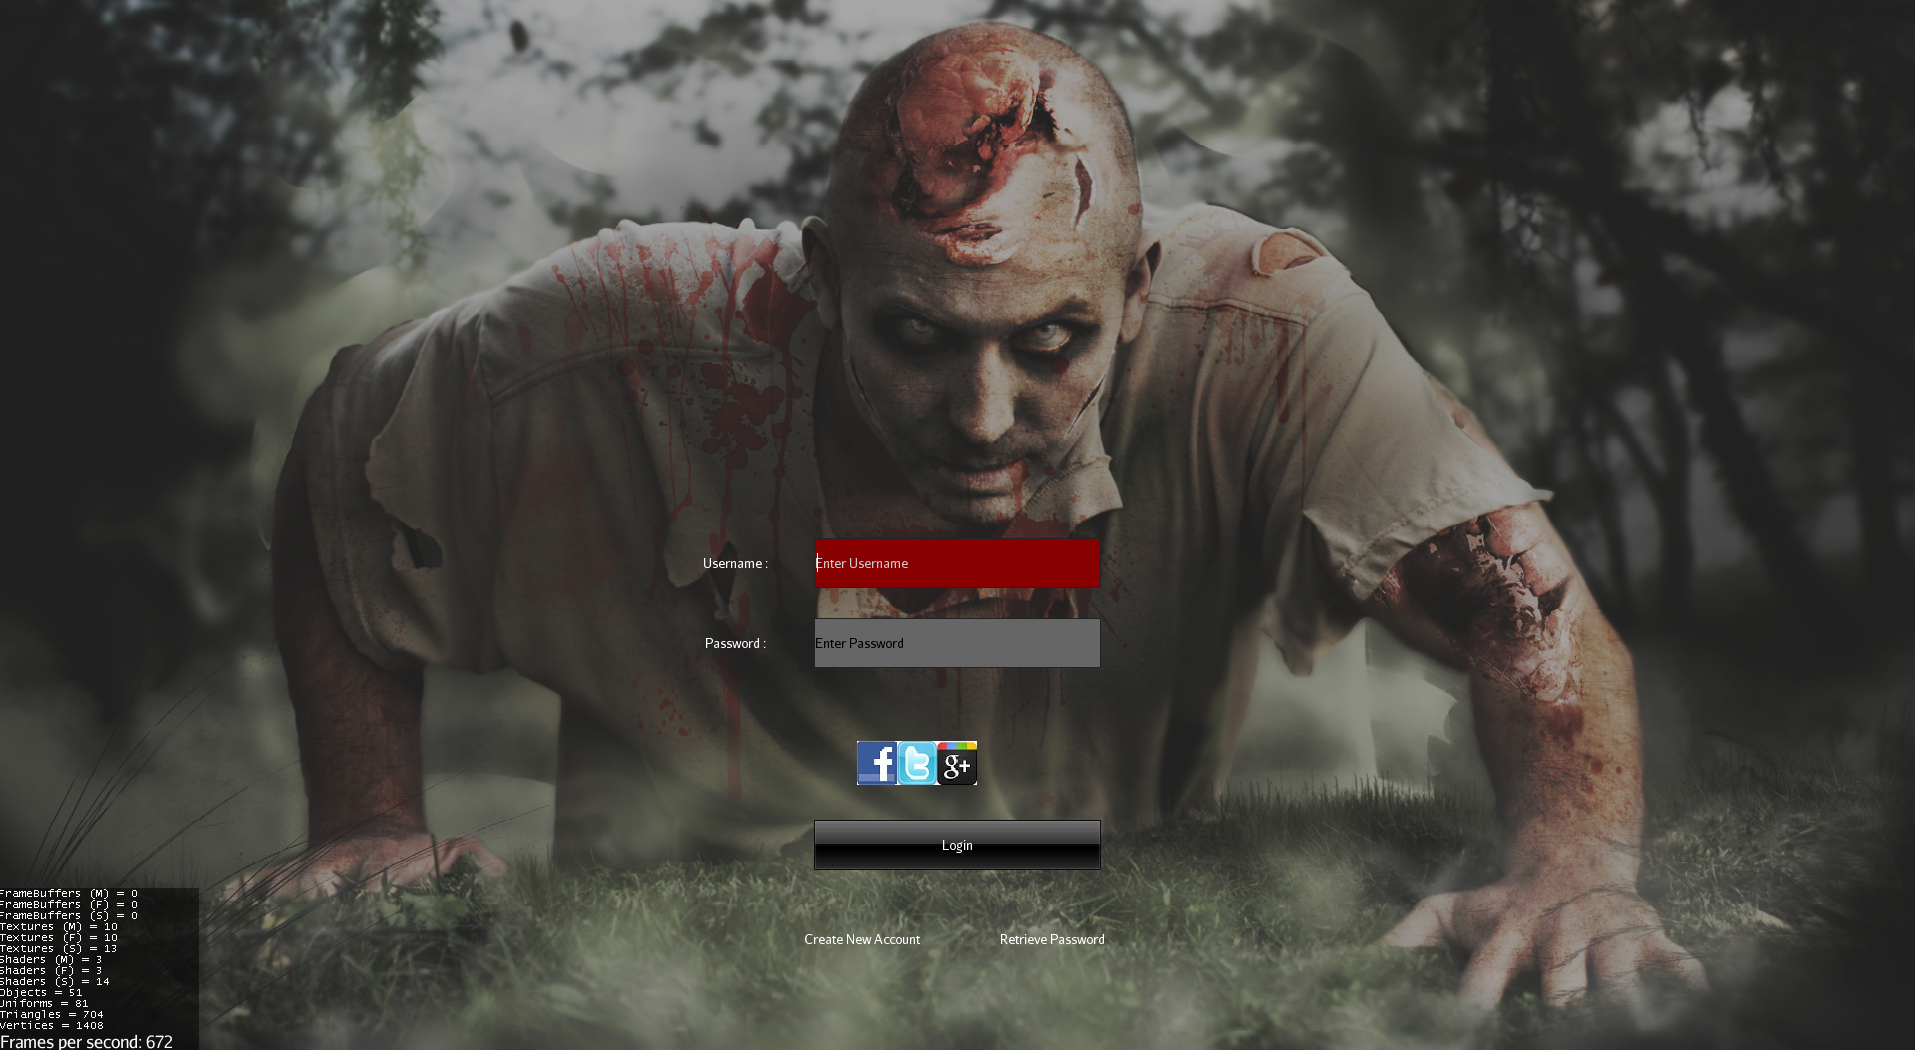
\includegraphics[width=130mm]		{GUI_ScreenShots/LoginScreen.jpg}
		\caption{Login Screen}
		\end{figure}
		

		
		\begin{figure}[H]
		\centering
		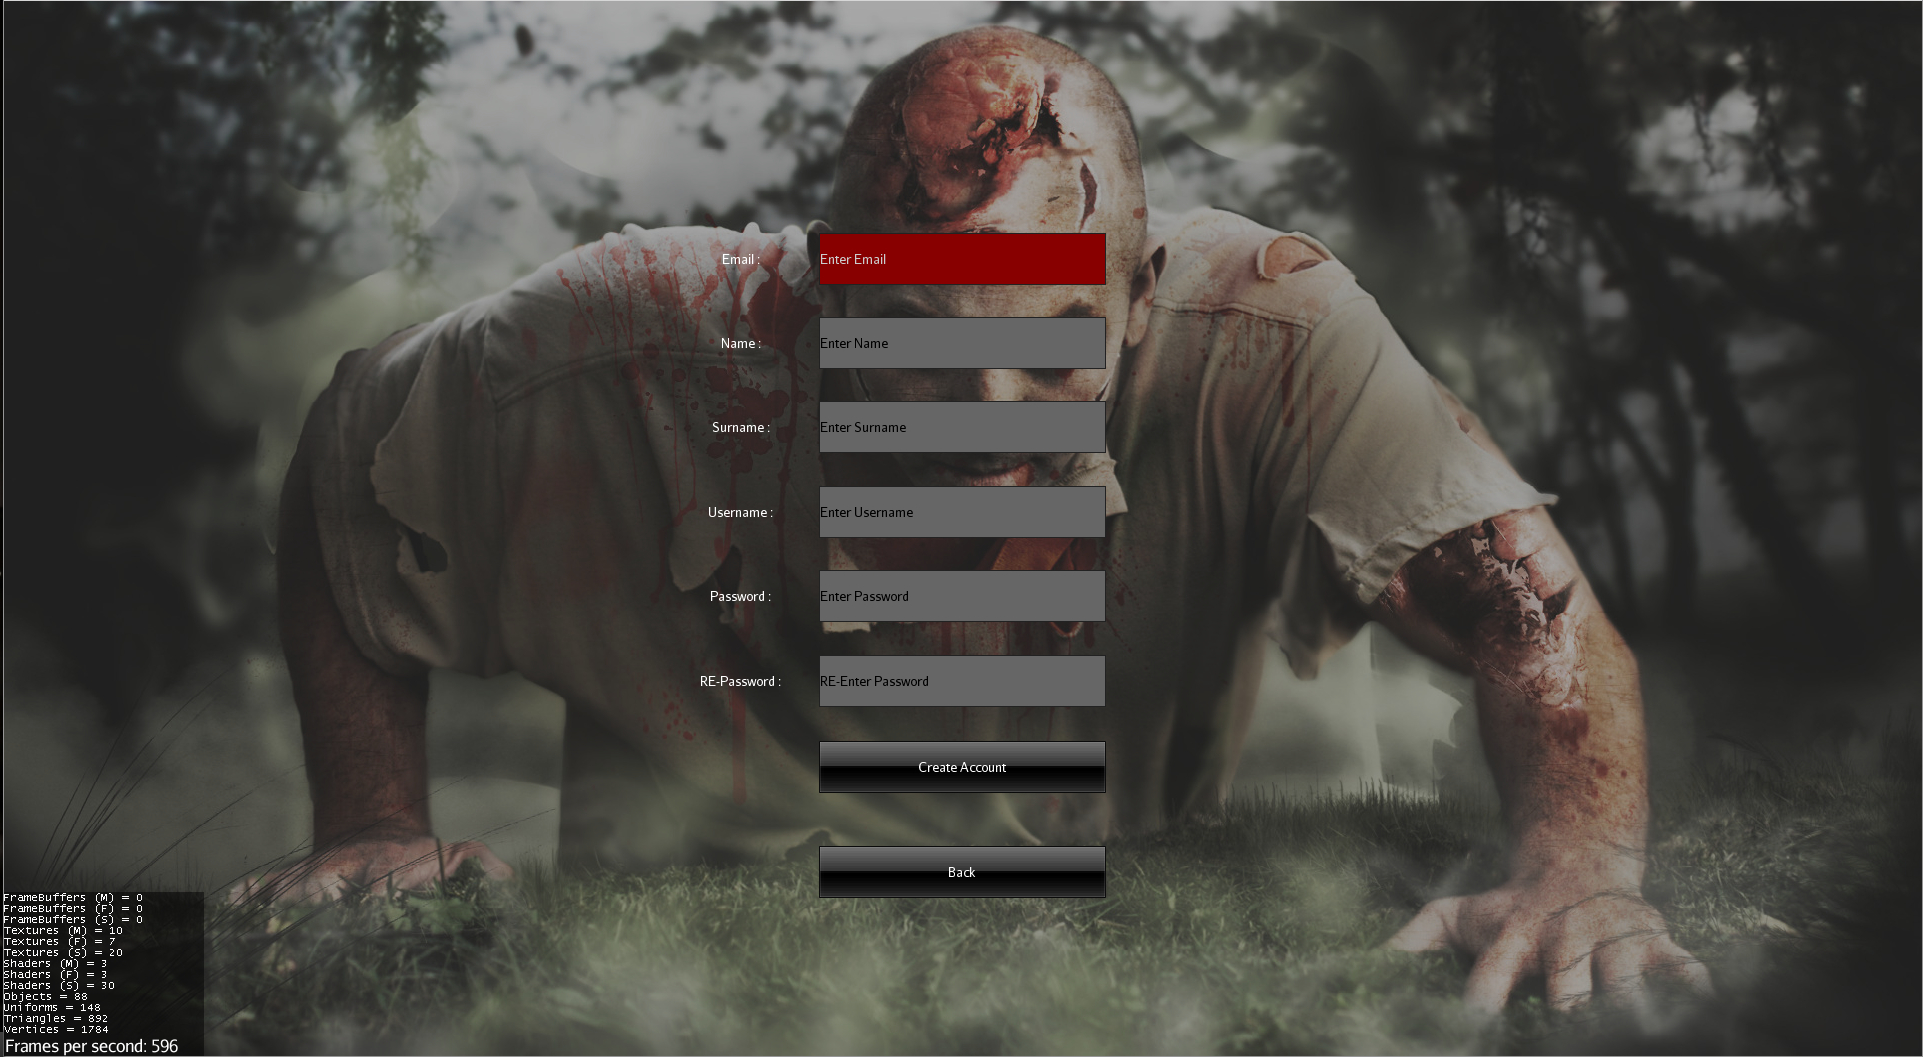
\includegraphics[width=130mm]{GUI_ScreenShots/CreateAccount.jpg}
		\caption{Create Account Screen}
		\end{figure}
		

			
		\begin{figure}[H]
		\centering
		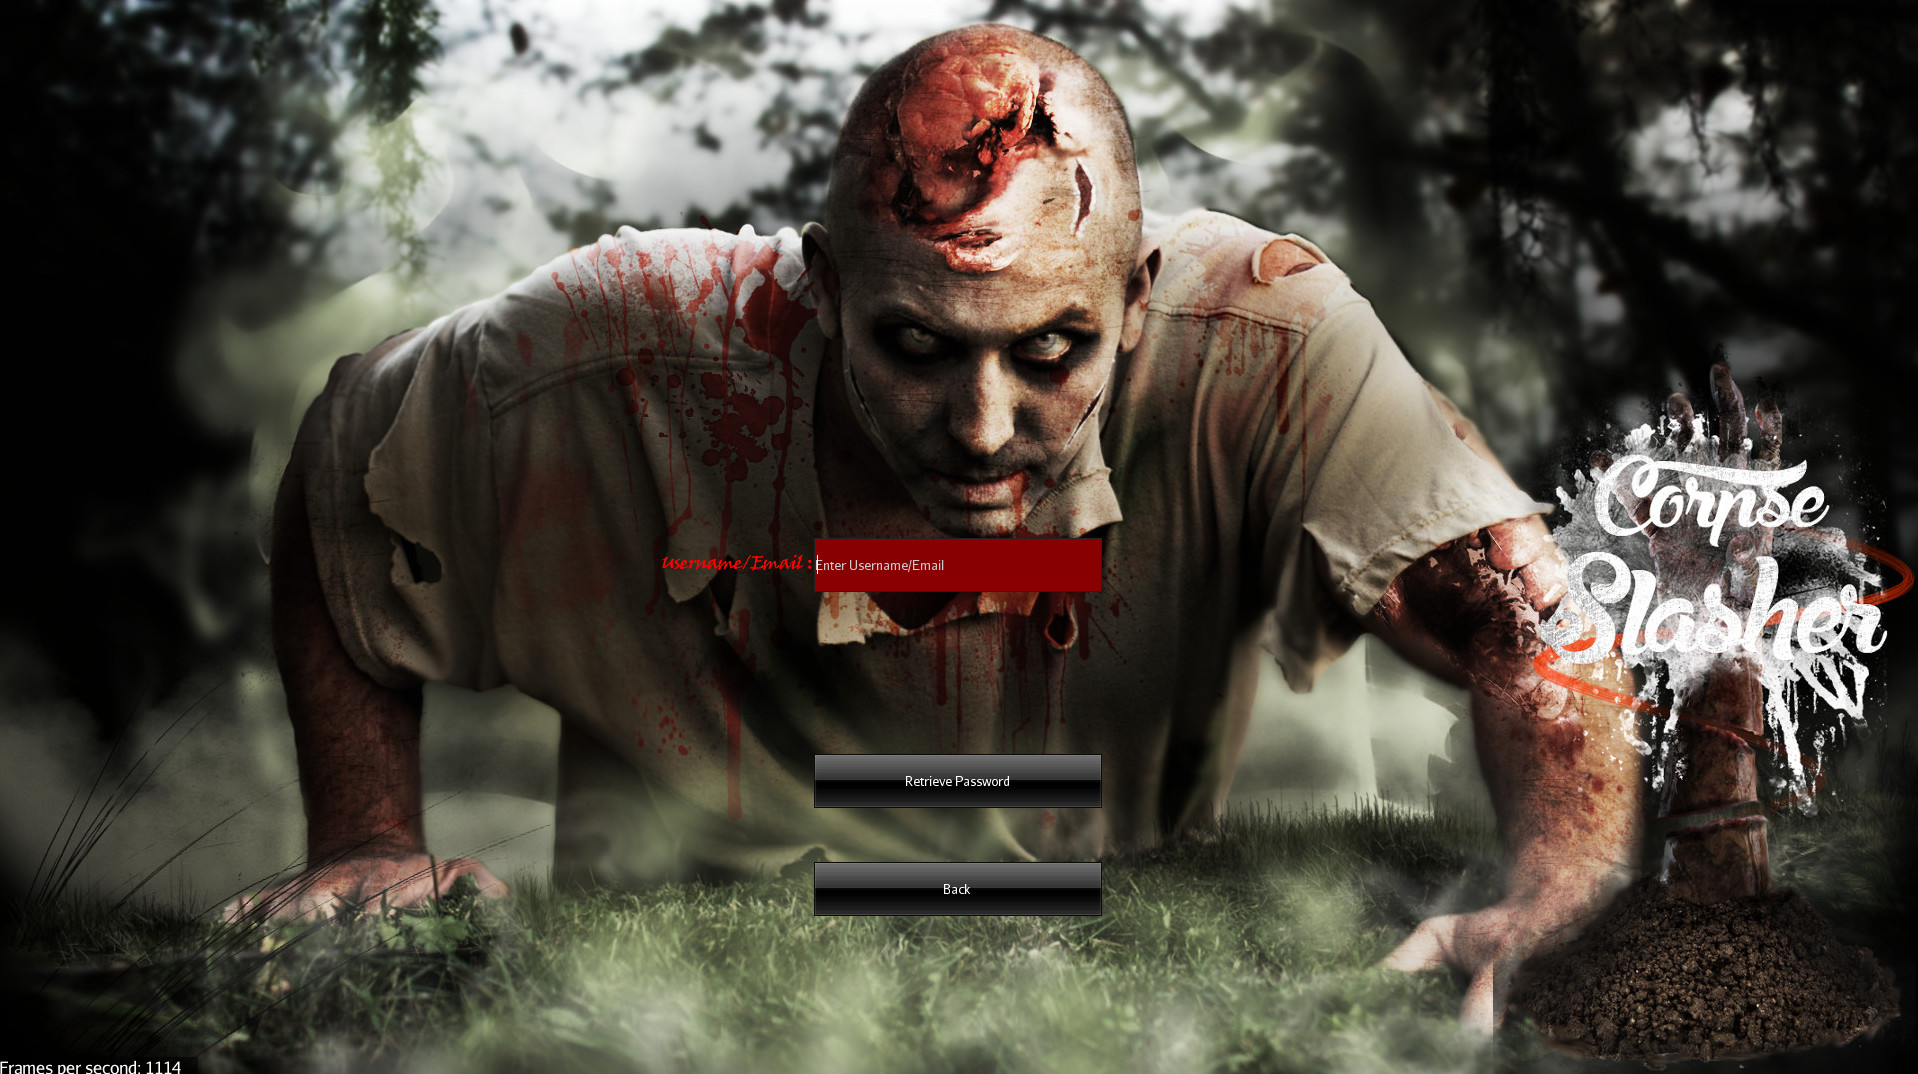
\includegraphics[width=130mm]{GUI_ScreenShots/RetrievePassword.jpg}
		\caption{Retrieve Password Screen}
		\end{figure}
		
			
		\begin{figure}[H]
		\centering
		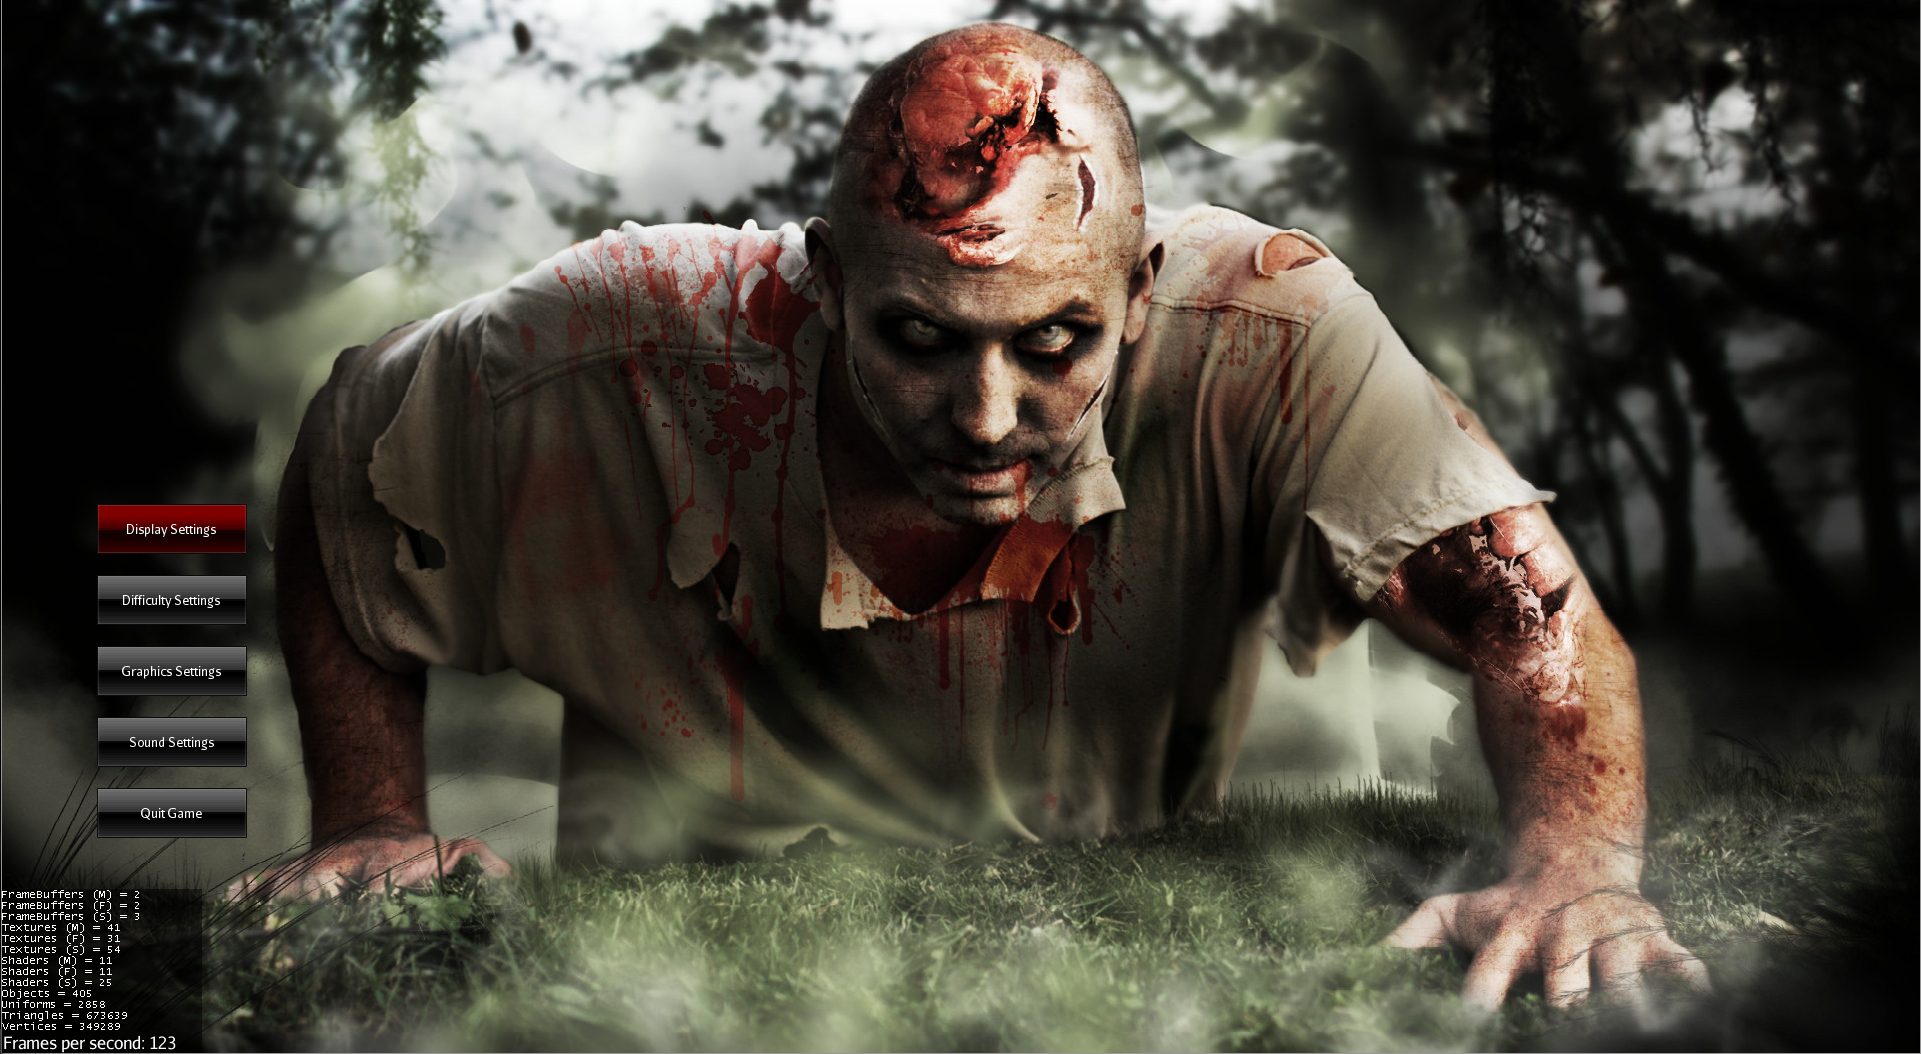
\includegraphics[width=130mm]{GUI_ScreenShots/OptionsScreen.jpg}
		\caption{Options Screen}
		\end{figure}
		
			
		\begin{figure}[H]
		\centering
		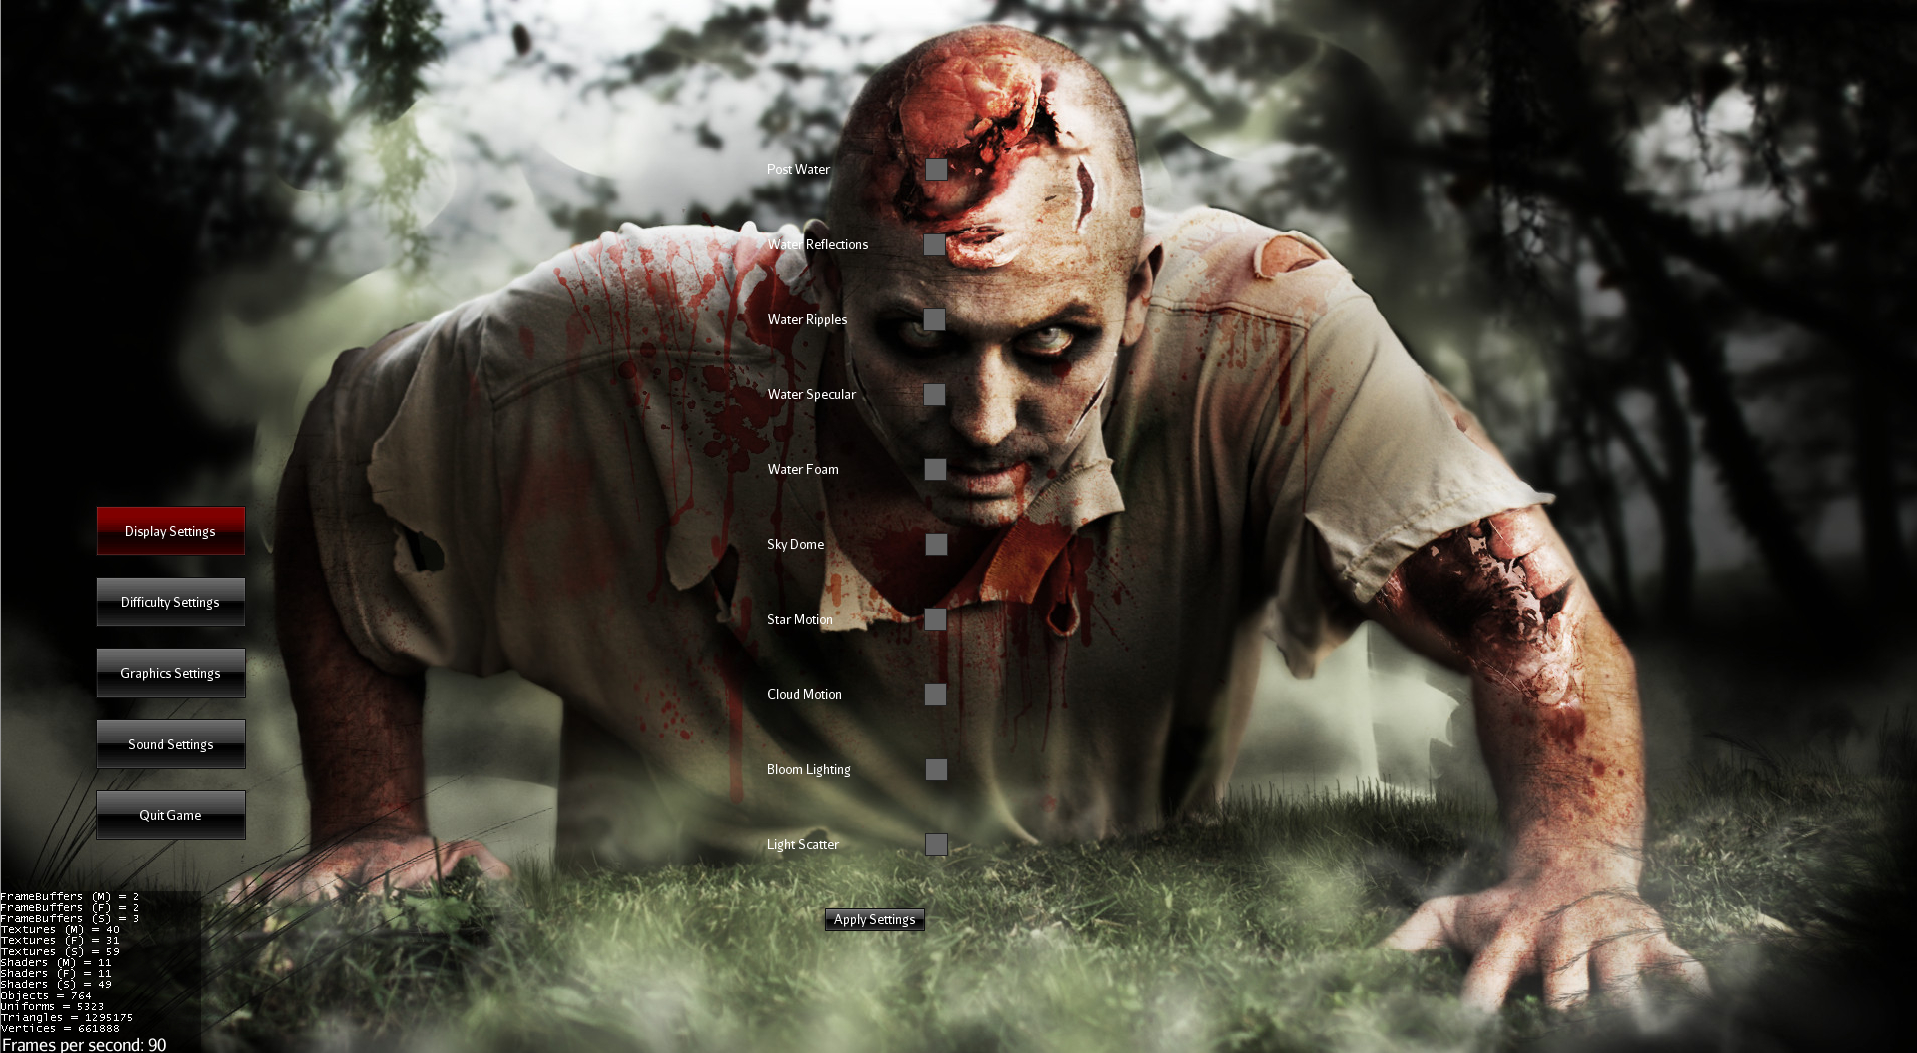
\includegraphics[width=130mm]{GUI_ScreenShots/GraphicsSettings.jpg}
		\caption{Graphics Settings tab}
		\end{figure}
		
		
		\vspace{0.2in}
\end{document}